\documentclass[a4paper,12pt,fleqn]{article}
%\documentclass[a4paper,12pt,twocolumn]{article}
\usepackage[margin=0.65in]{geometry}
\usepackage{fancyhdr}
\usepackage{amsmath,amsthm,amssymb,mathtools}
\usepackage{algorithm}% http://ctan.org/pkg/algorithm
\usepackage{algpseudocode}
\usepackage{graphicx}
\usepackage{hyperref}
\usepackage{breqn}
\usepackage{bbm}
\usepackage{lipsum}
\usepackage{epstopdf}
\usepackage[T1]{fontenc}
\usepackage[utf8]{inputenc}
\usepackage{ragged2e}
\usepackage{authblk}
\usepackage{enumitem}
\usepackage[stable]{footmisc}
\setlength{\mathindent}{0pt}
\def\Item$#1${\item $\displaystyle#1$
	\hfill\refstepcounter{equation}(\theequation)}
\def\ItemNN$#1${\item $\displaystyle#1$}
%usepackage[backend=bibtex,bibstyle=numeric,citestyle=numeric]{biblatex}
\usepackage[nottoc,numbib]{tocbibind}
\usepackage[round]{natbib}
\bibliographystyle{myplainnat}
\newcommand{\pkg}[1]{{\fontseries{b}\selectfont #1}} \newcommand{\diagentry}[1]{\mathmakebox[1.8em]{#1}}
\usepackage{nicefrac}
\usepackage[toc,page]{appendix}
\usepackage{array}
\usepackage{chngcntr}
\usepackage{ctable}
\counterwithin{table}{section}
\counterwithin{figure}{section}
\usepackage{multirow}
\usepackage[font=footnotesize]{caption}
\usepackage{subcaption}
\usepackage{graphicx}
\usepackage{float}
% command to number equations according to the their sections
\numberwithin{equation}{section}
\graphicspath{ {C:/Users/Windows/Dropbox/UCD/UCD_Staff/Publications/PCRC/} }
\usepackage{longtable}
\newcolumntype{L}[1]{>{\raggedright\let\newline\\\arraybackslash\hspace{0pt}}m{#1}}
\newcolumntype{C}[1]{>{\centering\let\newline\\\arraybackslash\hspace{0pt}}m{#1}}
\newcolumntype{R}[1]{>{\raggedleft\let\newline\\\arraybackslash\hspace{0pt}}m{#1}}
\usepackage{bbm}     %for the indicator function (but font type 3)
\usepackage{dsfont}  %for the indicator function (font type 1)
\newcommand{\indicator}[1]{\mathds{1}{\left( {#1} \right) }}
\def\given{\,|\,}
\newcolumntype{I}{% I for a thick rule
	!{\vline width 1.25pt}%
}

\title{Infinite Mixtures of Infinite Factor Analysers \\ \large Notes \& Derivations}
\author[1, 2]{Keefe Murphy}
\author[1, 2]{Dr. Claire Gormley}
\author[3]{Dr. Cinzia Viroli}
\affil[1]{School of Mathematics and Statistics, UCD}
\affil[2]{Insight Centre for Data Analytics, UCD}
\affil[3]{Department of Statistical Sciences, University of Bologna}
%\renewcommand\Authands{ and }

\date{}
\begin{document}
	\nocite{*}
	\maketitle
	%\begin{abstract}
	%\end{abstract}
	\newpage
	\begin{small}
	\tableofcontents
	\end{small}
	\begin{footnotesize}
		%\addcontentsline{toc}{section}{\listtablename}
		%\listoftables
		%\addcontentsline{toc}{section}{\listfigurename}
		%\listoffigures
	\end{footnotesize}
	\newpage
	
\section[Introduction]{Introduction}
\subsection[Background]{Background}
Modern clustering problems are increasingly high-dimensional, in the sense that the dimension of the feature vectors may be comparable to or even greater than the number of observations. In such cases, many common clustering techniques are known to perform poorly, and may even be intractable. We introduce a `choice-free' Bayesian nonparametric approach to fitting mixture models with a factor analytic structure, with particular focus on clustering $N \ll p$ datasets. In particular, we propose a suite of models of varying degress of complexity -- (Infinite) Factor Analysis (FA/IFA), Mixtures of (Infinite) Factor Analysers (MFA/MIFA), Overfitted Mixtures of (Infinite) Factor Analysers (OMFA/OMIFA), Infinite Mixtures of (Infinite) Factor Analysers (IMFA/IMIFA).

\subsection[Model Set-Up]{Model Set-Up}
Let $\underline{x} = \left(x_1, x_2, \ldots, x_p\right)^T$ have mean $\underline{\mu}$ and covariance matrix $\Sigma$. Orthogonal factor analysis is a Gaussian latent variable model, often used as a dimension reduction technique, under which $\underline{x}$ is linearly dependent upon a few $\left(q\ll{p}\right)$ unobservable random variables $\underline{\eta}_i$, called \textit{common factors} and $p$ additional sources of variation $\varepsilon_1,\varepsilon_2,\ldots,\varepsilon_p$ called \textit{specific factors}, for $i=1,\ldots,N$ observations, s.t.
\newline

\noindent\begin{tabular}{l l l l l l}
& $\underline{x}_i$ & $=$ & $\underline{\mu} + \Lambda\underline{\eta}_i + \underline{\varepsilon}_i$&\\
	\\
	where  & $\underline{x}_i$ & $\rightarrow$ & $\left(p \times 1\right)$ & observation vector \\
	& $\underline{\mu}$ &  $\rightarrow$ & $\left(p \times 1\right)$  & overall mean vector \\
	& $\Lambda$ &  $\rightarrow$ & $\left(p \times q\right)$  & loadings matrix \\
	& $\underline{\eta}_i$ &  $\rightarrow$ & $\left(q \times 1\right)$  & vector of factor scores for obs $i$ \\
	& $\underline{\varepsilon}_i$ & $\rightarrow$ & $\left(p \times 1\right)$  & vector of errors for obs $i$ \\
\end{tabular}
\\ \\
The \textit{factor loading} of the $j$-th variable on the $k$-th factor of the $\left(p \times q\right)$ matrix $\Lambda$ of factor loadings is denoted $\Lambda_{jk}$. If we assume the data have been centred to have column means of 0 then we have
\begin{equation}
\label{eq:1}
\left(\underline{x}_i - \underline{\mu}_{}\right)_{\left(p \times 1\right)} = \underline{x}_{i_{\left(p \times 1\right)}}^\star = \Lambda_{_{\left(p \times q\right)}}\underline{\eta}_{i_{\left(q \times 1\right)}} + \underline{\varepsilon}_{i_{\left(p \times 1\right)}}
\end{equation}

\subsection[Assumptions]{Assumptions}
\begin{enumerate}
	\item $\underline{\varepsilon}_i$ and $\underline{\eta}_i$ are independent, s.t. $\underline{\eta}_i~\perp\kern-7pt\perp\hspace{2mm}\underline{\epsilon}_i$ and $\mathrm{Cov}\left(\underline{\eta}_i,\underline{\varepsilon}_i\right) = \mathrm{E}\left(\underline{\eta}_i\underline{\varepsilon}_i^T\right) = 0$
	\item $\mathrm{E}\left(\underline{\varepsilon}_i\right) = \underline{0}$ and $ \mathrm{Cov}\left(\underline{\varepsilon}_i\right) = \begin{pmatrix}
	\diagentry{\psi_1} & 0 & \ldots & 0\\
	0 & \diagentry{\psi_2}& \ldots & 0\\
	\vdots & \vdots & \diagentry{\ddots}& \vdots\\
	0 & 0 & \ldots & \diagentry{\psi_p}
	\end{pmatrix} = \Psi$\\
	\begin{flalign}
	\label{eq:2}
	\therefore \underline{\varepsilon}_i \sim\textrm{MVN}_p\left(\underline{0},\Psi\right), \mbox{where $\Psi$ is a diagonal matrix whose non-zero elements}\nonumber&\\
	\psi_1,\ldots,\psi_p~\mbox{are known as \textit{uniquenesses}}&
	\end{flalign}
	\item $\mathrm{E}\left(\underline{\eta}_i\right) = \underline{0}$ and $ \mathrm{Cov}\left(\underline{\eta}_i\right) = \begin{pmatrix}
	\diagentry{1} & 0 & \ldots & 0\\
	0 & \diagentry{1}& \ldots & 0\\
	\vdots & \vdots & \diagentry{\ddots}& \vdots\\
	0 & 0 & \ldots & \diagentry{1}
	\end{pmatrix} = \mathcal{I}_q$
	\begin{equation}
	\label{eq:3}
	\therefore \underline{\eta}_i \sim \textrm{MVN}_q\left(\underline{0}, \mathcal{I}_q\right)
	\end{equation}
\end{enumerate}

\section[Bayesian Framework]{Bayesian Framework}
\subsection[Likelihood]{Likelihood}
\begin{flalign}
	\mathrm{E}\left(\underline{x}_i^\star\right) & = \mathrm{E}\left(\Lambda\underline{\eta}_i + \underline{\varepsilon}_i\right) \nonumber&\\
	& = \Lambda\mathrm{E}\left(\underline{\eta}_i\right) + \mathrm{E}\left(\underline{\varepsilon}_i\right) \nonumber&\\
	& = \underline{0} \nonumber&\\
	\label{eq:4}
	\therefore \underline{x}_i^\star & \sim   \textrm{MVN}_p\left(\underline{0},\Sigma\right)&\\
	\nonumber\\
	\mbox{Since} \hspace{2mm}  \underline{\varepsilon}_i & = \underline{x}_i^\star -\Lambda\underline{\eta}_i,\nonumber&\\
	\Sigma & = \mathrm{Cov}\left(x_i\right)\nonumber&\\
	& = \mathrm{E}\left[\left(\underline{x}_i-\underline{\mu}_i\right)\left(\underline{x}_i-\underline{\mu}_i\right)^T\right]\nonumber&\\
	& = \mathrm{E}\left[\underline{x}_i^\star \underline{x}_i^{\star^{T}}\right]\nonumber&\\
	& =  \mathrm{E}\left[\left(\Lambda\underline{\eta}_i+\underline{\varepsilon}_i\right)\left(\Lambda\underline{\eta}_i+\underline{\varepsilon}_i\right)^T\right]\nonumber&\\
	& =  \mathrm{E}\left[\left(\Lambda\underline{\eta}_i\right) +
	\underline{\varepsilon}_i\left(\Lambda\underline{\eta}_i\right)^T + \left(\Lambda\underline{\eta}_i\right)\underline{\varepsilon}_i^T + \underline{\varepsilon}_i\underline{\varepsilon}_i^T\right]\nonumber&\\
	& = \Lambda\mathrm{E}\left(\underline{\eta}_i\underline{\eta}_i^T\right)\Lambda^T + \mathrm{E}\left(\underline{\varepsilon}_i\underline{\eta}_i^T\right)\Lambda^T + \Lambda\mathrm{E}\left(\underline{\eta}_i\underline{\varepsilon}_i^T\right) + \mathrm{E}\left(\underline{\varepsilon}_i\underline{\varepsilon}_i^T\right)\nonumber&\\
	& = \Lambda\Lambda^T + \Psi \nonumber&\\
	\label{eq:5} \therefore \underline{x}_i^\star & \sim  \textrm{MVN}_p\left(\underline{0},\Lambda\Lambda^T + \Psi\right)&\\
	\nonumber\\
	\mathrm{E}\left(\underline{x}_i^\star \given \underline{\eta}_i\right) & = \mathrm{E}\left(\Lambda\underline{\eta}_i + \underline{\varepsilon}_i \given \underline{\eta}_i\right)\nonumber\\
	& =	\Lambda\mathrm{E}\left(\underline{\eta}_i \given \underline{\eta}_i\right) + \mathrm{E}\left(\underline{\varepsilon}_i \given \underline{\eta}_i\right)\nonumber&\\
	& = \Lambda\underline{\eta}_i\nonumber&\\
	\mathrm{Cov}\left(\underline{x}_i^\star \given \underline{\eta}_i\right) & = \mathrm{E}\left[\left(\underline{x}_i^\star - \Lambda\underline{\eta}_i\right)\left(\underline{x}_i^\star - \Lambda\underline{\eta}_i\right)^T \given \underline{\eta}_i\right]\nonumber&\\
	& = \mathrm{E}\left(\underline{\varepsilon}_i\underline{\varepsilon}_i^T \given \underline{\eta}_i\right)\nonumber&\\
	& = \Psi\nonumber&\\
	\label{eq:6} \therefore \underline{x}_i^\star \given \underline{\eta}_i & \sim  \textrm{MVN}_p\left(\Lambda\underline{\eta}_i,\Psi\right)&\\
	\intertext{The density of the data is then given by:}
	\label{eq:7}\mathrm{P}\left(\underline{x}_i^\star 
	\given \underline{\eta}_i, \Lambda,\Psi\right) & = \left(2\pi\right)^{-\frac{p}{2}} 
	\given\Psi\given^{-\frac{1}{2}} \exp\left(-\frac{1}{2}\sum_{i=1}^{N}\left(\underline{x}_i^\star - \Lambda\underline{\eta}_i\right)^T\Psi^{-1}\left(\underline{x}_i^\star - \Lambda\underline{\eta}_i\right)\right)&\\
	& \propto \given\Psi\given^{-\frac{1}{2}} \exp\left(-\frac{1}{2}\mathrm{tr}\left[\Psi^{-1}\left(X - \eta\Lambda\right)^T\left(X - \eta\Lambda\right)\right]\right)\nonumber&\\
	\mbox{where} \hspace{2mm} \Lambda_{\left(p \times q\right)} & = \begin{pmatrix}
	\diagentry{\lambda_{11}} & \lambda_{12} & \ldots & \lambda_{1q}\\
	\lambda_{21} & \diagentry{\lambda_{22}}& \ldots & \lambda_{2q}\\
	\vdots & \vdots & \diagentry{\ddots}& \vdots\\
	\lambda_{p1} & \lambda_{p2} & \ldots & \diagentry{\lambda_{pq}}
	\end{pmatrix}\nonumber&\\
	\& \hspace{2mm} \eta_{\left(N \times q\right)} & = \begin{pmatrix}
	\diagentry{\eta_{11}} & \eta_{12} & \ldots & \eta_{1q}\\
	\eta_{21} & \diagentry{\eta_{22}}& \ldots & \eta_{2q}\\
	\vdots & \vdots & \diagentry{\ddots}& \vdots\\
	\eta_{N1} & \eta_{N2} & \ldots & \diagentry{\eta_{Nq}}
	\end{pmatrix} \& \hspace{2mm}\underline{\eta}_i \hspace{2mm} 
	\mbox{is a column vector containing the entries of row $i$ of $\eta$}\nonumber&
\end{flalign}

\subsection[Posterior Set-Up]{Posterior Set-Up}
\begin{flalign}
	\mbox{Likelihood} \hspace{2mm} &= \prod_{i=1}^N\mathrm{P}\left(\underline{x}_i^\star \given \underline{\eta}_i, \Lambda,\Psi\right)\nonumber&\\
	\label{eq:8}
	\mbox{where}~\mathrm{P}\left(\underline{x}_i^\star \given \underline{\eta}_i, \Lambda,\Psi\right) &\sim  \textrm{MVN}_p\left(\Lambda\underline{\eta}_i,\Psi\right)&\\
	\mbox{Prior} \hspace{2mm}&= \mathrm{P}\left(\eta\right)\mathrm{P}\left(\Lambda\right)\mathrm{P}\left(\Psi\right)\nonumber &\\
	 \mbox{Posterior} \hspace{2mm} &= \mbox{Likelihood} \times \mbox{Prior}&\nonumber\\
	 \therefore \mathrm{P}\left(\eta, \Lambda,\Psi
	  \given X^\star\right) 
	  &\propto \mathcal{L}\left(X^\star \given \eta, \Lambda, \Psi\right) \mathrm{P}\left(\eta\right)\mathrm{P}\left(\Lambda\right)\mathrm{P}\left(\Psi\right)\nonumber&\\
	  &\label{eq:9}\propto \left[\prod_{i=1}^{N}\mathrm{P}\left(\underline{x}_i^\star \given \underline{\eta}_i, \Lambda,\Psi\right)\right]
	  \left[\prod_{i=1}^{N}\mathrm{P}\left(\underline{\eta}_i\right)\right] \left[\prod_{j=1}^{p}\mathrm{P}\left(\underline{\Lambda}_j\right)\right]\left[\prod_{j=1}^{p}\mathrm{P}\left(\psi_j\right)\right]&
	 \end{flalign}
	 
Later on, especially as we move into the mixture case, it will be necessary to undo the centering, thereby removing the $^\star$ on $\underline{x}_i^\star$,  and reintroduce $\underline{\mu}$. This will necessitate multiplying the quantity in \eqref{eq:9} by $\mathrm{P}\left(\underline{\mu}\right)$. However, we will proceed to derive the full conditionals we need for Gibbs Sampling using the centered notation for now as adjusting for $\underline{\mu}$ afterwards will be trivial.
\newpage

\section[Sampling from the Full Conditionals]{Sampling from the Full Conditionals}
\subsection[Factor Scores]{Factor Scores - $\underline{\eta}_i$}
\begin{flalign}
\underline{\eta}_i &\sim\textrm{MVN}_q\left(\underline{0}, \mathcal{I}_q\right)\nonumber&\\
\label{eq:10}& = \left(2\pi\right)^{-\frac{q}{2}}\exp\left(-\frac{1}{2}\underline{\eta}_i^T\underline{\eta}_i\right)&
\end{flalign}
To obtain the full conditional for $\underline{\eta}_i$ we can multiply the likelihood by the prior in \eqref{eq:10} s.t.
\begin{flalign}
\mathrm{P}\left(\underline{\eta}_i \given , \underline{x}_i^\star,\Lambda,\Psi\right) &\sim \mathrm{P}\left(\underline{x}_i^\star \given \underline{\eta}_i, \Lambda,\Psi\right)\mathrm{P}\left(\underline{\eta}_i\right)\nonumber&\\
& \propto \exp\left(-\frac{1}{2}\left[\left(\underline{x}_i^\star - \Lambda\underline{\eta}_i\right)^T\Psi^{-1}\left(\underline{x}_i^\star - \Lambda\underline{\eta}_i\right) + \underline{\eta}_i^T\underline{\eta}_i\right]\right)\nonumber&\\
& \propto \exp\left(-\frac{1}{2}\left[-\underline{x}_i^{\star^ {T}}\Psi^{-1}\Lambda\underline{\eta}_i 
	  - \left(\Lambda\underline{\eta}_i\right)^T\Psi^{-1}\underline{x}_i^\star 
	  + \left(\Lambda\underline{\eta}_i\right)^T\Psi^{-1}\left(\Lambda\underline{\eta}_i\right)
	  + \underline{\eta}_i^T\underline{\eta}_i\right]\right)\nonumber&\\
\label{eq:11}& \propto \exp\left(-\frac{1}{2}
	  \left\{\underline{\eta}_i^T\left[\mathcal{I}_q + \Lambda^T\Psi^{-1}\Lambda\right]\underline{\eta}_i\right\} + \underline{x}_i^{\star^ {T}}\Psi^{-1}\Lambda\underline{\eta}_i \right)&\\
	  \intertext{As this is the product of two $\textrm{MVN}$ distributions we can expect the result to also be $\textrm{MVN}$.\newline Typically,}
	  \textrm{MVN}\left(\mu,\Sigma\right) & \propto \exp\left(-\frac{1}{2}\left(\underline{x}-\underline{\mu}\right)^T\Sigma^{-1}\left(\underline{x}-\underline{\mu}\right)\right)\nonumber&\\
& = \exp\left(-\frac{1}{2}\left(\underline{x}^T\Sigma^{-1}\underline{x} -2\underline{\mu}^T\Sigma^{-1}\underline{x} + \underline{\mu}^T\underline{\Sigma}^{-1}\underline{\mu}\right)\right)\nonumber&
\label{eq:12}\intertext{We can identify the $\mu$ and $\Sigma^{-1}$ terms from \eqref{eq:11} above to yield} 
\mathrm{P}\left(\underline{\eta}_i \given \underline{x}_i^\star,\Lambda,\Psi\right) &\sim  \textrm{MVN}_q\left(\left[\mathcal{I}_q + \Lambda^T\Psi^{-1}\Lambda\right]^{-1}\Lambda^T\Psi^{-1}\underline{x}_i^\star,\left[\mathcal{I}_q + \Lambda^T\Psi^{-1}\Lambda\right]^{-1}\right)&
\end{flalign}
\noindent However, we can reintroduce $\underline{\mu}$ and save on computational time if we implement the algorithm of \citet{GMRFbook}\footnote{To sample $x\sim\textrm{N}\left(\mu, \Omega^{-1}\right)$, find a matrix $U$ -- non-unique, and square or `tall' -- via Cholesky Decomposition s.t. $U^TU=\Omega$, sample from $z\sim\textrm{N}\left(0, 1\right)$, then backsolve $L^Tv = Uv = z$ s.t $x=\mu+v=\mu+L^{-T}z=\mu+U^{-1}z.$ Then$\colon$\begin{itemize}\item $\mathrm{E}\left(x\right)= \mu + U^{-1}\mathrm{E}\left(z\right)=\mu$\item $\mathrm{Cov}\left(x,x\right)=\mathrm{Cov}\left(L^{-T},z\right)=\left(L^TL\right)^{-1}=\Omega^{-1}$\end{itemize}}. In fact, we can extend this to block update the scores, thereby obviating the need to loop over $i$:
\begin{itemize}
	\item Calculate $\Omega_\eta = \mathcal{I}_q + \Lambda^T\Psi^{-1}\Lambda$
	\item Compute the Cholesky Factorization $\Omega_\eta = U^TU$.
	\item Sample $\underline{z} \sim \textrm{MVN}_q\left(\underline{0}, \mathcal{I}_q\right)~N$ times.
	\item Backsolve $U\underline{v} = \underline{z}^T$.
	\item Compute $\Omega_\eta^{-1}$ from $U$.
	\Item $\mbox{Return}~\left(\Omega_\eta^{-1}\Lambda^T\Psi^{-1}\left(C_n\underline{\mu}X\right)^T + \underline{v}\right)^T$\newline where $C_n = \mathcal{I}_n - \frac{1}{n}\mathcal{O} $ and $\mathcal{O}$ is an $N\times N$ matrix of all $1$'s. \label{eq:13}
	\end{itemize}

\subsection[Loadings Matrix]{Loadings Matrix - $\Lambda$}
\label{Loadings_Section}A Gaussian distribution is a conjugate prior for $\Lambda$, thus an $\textrm{MVN}_q$ distribution prior is assumed for each row $\underline{\Lambda}_j$ of $\Lambda$ s.t. $\underline{\Lambda}_j \sim \textrm{MVN}_q\left(\underline{0},\Sigma_{\lambda}\right)$ where $\Sigma_{\lambda}$ is a diagonal covariance matrix. As above, we can expect the result of the product of two $\textrm{MVN}_q$ distributions to itself be distributed this way.
\begin{flalign}
\mathrm{P}\left(\underline{\Lambda}_j\given X^\star,\eta,\Psi\right) &\sim \mathrm{P}\left(X^\star \given \eta, \underline{\Lambda}_j,\Psi\right)\mathrm{P}\left(\underline{\Lambda}_j\given\Sigma_{\lambda}\right)\nonumber&\\
& \propto \exp\left(-\frac{1}{2}\sum_{i=1}^{N}\left(\underline{x}_i^\star - \underline{\Lambda}_j\underline{\eta}_i\right)^T\psi_j^{-1}\left(\underline{x}_i^\star - \underline{\Lambda}_j\underline{\eta}_i\right)\right)\exp\left(-\frac{1}{2}\left(\underline{\Lambda}_j^T\Sigma_{\lambda}^{-1}\underline{\Lambda}_j\right)\right) \nonumber&\\
& \propto \exp\left(-\frac{1}{2}\sum_{i=1}^{N}\left[- 2\underline{x}_i^{\star^{T}}\psi_j^{-1}\left(\underline{\Lambda}_j\underline{\eta}_i\right) + \left(\underline{\Lambda}_j\underline{\eta}_i\right)^T\psi_j^{-1}\left(\underline{\Lambda}_j\underline{\eta}_i\right) + \underline{\Lambda}_j^T\Sigma_{\lambda}^{-1}
\underline{\Lambda}_j\right]\right)\nonumber&\\
& \propto \exp\left(\underline{\Lambda}_j\psi_j^{-1}\sum_{i=1}^{N}x_{ij}^{\star^{T}}\underline{\eta}_i - \frac{1}{2}\underline{\Lambda}_j^T\left[\sum_{i=1}^{N}\psi_j^{-1}\underline{\eta}_i^T\underline{\eta}_i\right]\underline{\Lambda}_j -\frac{1}{2} \underline{\Lambda}_j^T\Sigma_{\lambda}^{-1}\underline{\Lambda}_j\right)\nonumber&\\
\label{eq:14}& \propto \exp\left(\underline{\Lambda}_j\left[\eta^T\psi_j^{-1}\underline{x}^{j^\star}\right] - \frac{1}{2}\underline{\Lambda}_j^T\left[\Sigma_{\lambda}^{-1} + \psi_j^{-1}\eta^T\eta\right]\underline{\Lambda}_j\right)&
\end{flalign}
where $\underline{x}^{j^\star}$ is an $N$-vector containing the elements of the $j$-th column of $X^\star$.
\begin{equation}
\begin{split}
	\therefore \mathrm{P}\left(\underline{\Lambda}_j\given X^\star,\eta,\Psi\right) &\sim&\hspace{-3mm} \textrm{MVN}_q\Big(\left[\Sigma_{\lambda}^{-1} + \psi_j^{-1}\eta^T\eta\right]^{-1}\eta^T\psi_j^{-1}\underline{x}^{j^\star},\\&&\left[\Sigma_{\lambda}^{-1} + \psi_j^{-1}\eta^T\eta\right]^{-1}\Big)&\label{eq:15}
\end{split}
\end{equation}
\noindent However, we can reintroduce $\underline{\mu}$ and save on computational time, as before, if we:
\begin{itemize}
	\item Calculate $\Omega_{\lambda_j} = \Sigma_{\lambda}^{-1} + \psi_j^{-1}\eta^T\eta$.
	\item Compute the Cholesky Factorization $\Omega_{\lambda_j} = U^TU$.
	\item Sample $\underline{z} \sim \textrm{MVN}_q\left(\underline{0}, \mathcal{I}_q\right)$.
	\item Back-solve $U\underline{v} = \underline{z}$.
	\item Compute $\Omega_{\lambda_j}^{-1}$ from $U$.
	\Item $\mbox{Return}~\Omega_{\lambda_j}^{-1}\eta^T\psi_j^{-1}\left(\underline{x}^{j} - \underline{1}\mu_j\right) + \underline{v}$\newline
	where $\underline{1}$ is an $N$-vector of all $1$'s. \label{eq:16}
\end{itemize}

\subsection[Uniquenesses]{Uniquenesses - $\Psi$}
\begin{flalign}
\shortintertext{If we assume an Inverse Wishart prior distribution for $\Psi$, we have:}
\mathrm{P}\left(\Psi\right) & \propto \given\Psi^{-1}\given^{\frac{N + p + 1}{2}}\exp\left(-\frac{1}{2}\mathrm{tr}\left(\mathcal{S}^{-1^\star}\Psi\right)\right)&\nonumber\\
\shortintertext{Using the fact that
$\mathrm{V}^{-1} \sim \textrm{Wish}_p\left(\nu, \Sigma\right)~\mbox{when}~ \mathrm{V} \sim \textrm{Wish}_p^{-1}\left(m, \Sigma^{-1}\right)~\mbox{with}~m = \nu + p + 1$ we get:}
\mathrm{P}\left(\Psi^{-1}\right) & \propto \given\Psi^{-1}\given^{\frac{N}{2}}\exp\left(-\frac{1}{2}\mathrm{tr}\left(\mathcal{S}^\star\Psi^{-1}\right)\right)\nonumber
\shortintertext{Since $\Psi$ is a diagonal matrix$\colon$}
\mathrm{P}\left(\Psi^{-1}\right) & \propto \prod_{j=1}^{p}\given\psi_j^{-1}\given^{\frac{N}{2}}\exp\left(-\frac{1}{2}\mathrm{tr}\left(\mathcal{S}_j^\star\psi_j^{-1}\right)\right)\nonumber
\shortintertext{This suggests the prior for $\Psi^{-1}$ is a product of $p \hspace{2mm} \textrm{Ga}\left(\alpha,\beta\right)$ distributions. We choose hyperparameters as per \citet{Fruhwirth-Schnatter2010-II}, by bounding each $\psi_j$ away from zero in such a way that Heywood problems are avoided, with a sufficiently large shape $\alpha$ and variable-specific rate hyperparameters $\beta_j$ derived from $\left(\mathbf{S}^{-1}\right)_{jj}$ or, if $p\geq N$, $\left(\mathbf{S}_{jj}\right)^{-1}$.}
\therefore \mathrm{P}\left(\Psi^{-1} \given \alpha, \beta_j \right) & = \prod_{j=1}^{p}\mathrm{P}\left(\psi_j^{-1} \given \alpha, \beta_j \right)&\nonumber \\
& \propto \prod_{j=1}^{p} \left(\psi_j^{-1}\right)^{\alpha - 1}\exp\left(- \beta_j\psi_j^{-1}\right)\nonumber&\\
\therefore \mathrm{P}\left(\Psi^{-1}\given X^\star, \eta, \Lambda\right) &\propto \mathrm{P}\left(X^\star \given \eta,\Lambda\right)\mathrm{P}\left(\Psi^{-1} \given \alpha,\beta_j\right) \nonumber&\\
&\propto \prod_{j=1}^{p}\left(\psi_j^{-1}\right)^{\frac{N}{2}}\exp\left(-\frac{\mathcal{S}_j^\star}{2}\psi_j^{-1}\right)\prod_{j=1}^{p}\left(\psi_j^{-1}\right)^{\alpha - 1}\exp\left(-\beta_j\psi_j^{-1}\right)\nonumber&\\
& \propto \prod_{j=1}^{p}\left(\psi_j^{-1}\right)^{\frac{N}{2} + \alpha - 1}\exp\left(-\bigg(\frac{\mathcal{S}_j^\star}{2} + \beta_j\bigg)\psi_j^{-1}\right)\label{eq:17}\\
\mbox{where} \hspace{2mm}\mathcal{S}_j^\star &=  \sum_{i=1}^{N}\left(x_{ij} - \underline{\Lambda}_j\underline{\eta}_i\right)^2\nonumber 
\shortintertext{However, we can reintroduce $\underline{\mu}$ at this stage by rewriting:}
\mathcal{S}_j &=  \sum_{i=1}^{N}\left(x_{ij} - \mu_j - \underline{\Lambda}_j\underline{\eta}_i\right)^2 \nonumber&
\shortintertext{Thus the posterior distribution of each $\psi_j^{-1}$ is given by:}
\mathrm{P}\left(\psi_j^{-1}\given X,F,\Lambda\right) & \sim \textrm{Ga}\left(\alpha + \frac{N}{2},\beta_j + \frac{S_j}{2}\right)&\label{eq:18}
\end{flalign}
\subsection[Reintroducing $\mu$]{Reintroducing $\underline{\mu}$}
We've already seen from \eqref{eq:13}, \eqref{eq:16} and \eqref{eq:18} that reintroducing $\underline{\mu}$ to the other full conditionals is trivial. All that remains is to specify the conjugate Gaussian prior for $\underline{\mu}$ itself, and to derive its full conditional. We assume an $\textrm{MVN}_p$ distribution as a prior s.t. $\underline{\mu} \sim \textrm{MVN}_p\left(\underline{\tilde{\mu}}, \Sigma_{\mu}\right)$ where $\Sigma_{\mu}$ is a diagonal covariance matrix, typically the diagonal of the data's sample covariance matrix, and $\underline{\tilde{\mu}}$ is a vector of prior mean means, typically the sample mean. In the mixture case, this will be the sample mean of each initialised group. As above, we can expect the result of the product of two $\textrm{MVN}_p$ distributions to itself be distributed this way.
\begin{flalign}
\mathrm{P}\left(\underline{\mu}\given X,\eta,\Psi, \Lambda\right)
& \propto  \exp\left(-\frac{1}{2}\sum_{i=1}^{N}\left(\underline{x}_i - \underline{\mu} - \Lambda\underline{\eta}_i\right)^T\Psi^{-1}\left(\underline{x}_i - \underline{\mu} - \Lambda\underline{\eta}_i\right)\right)\exp\left(-\frac{1}{2}\left(\underline{\mu} - \underline{\tilde{\mu}}\right)^T\Sigma_{\mu}^{-1}\left(\underline{\mu} - \underline{\tilde{\mu}}\right)\right) \nonumber&\\
& \propto \exp\left(-\frac{1}{2}\bigg(\sum_{i=1}^{N}\left[-2 \underline{x}_i^T\Psi^{-1}\underline{\mu} + 2\left(\Lambda\underline{\eta}_i\right)^T\Psi^{-1}\underline{\mu}  + \underline{\mu}^T\Psi^{-1}\underline{\mu}\right] +\underline{\mu}^T \Sigma_{\mu}^{-1}\underline{\mu} - 2\underline{\tilde{\mu}}^T\Sigma_{\mu}^{-1}\underline{\mu}\bigg)\right)\nonumber&\\
& \propto  \exp\left(\sum_{i=1}^{N}\underline{x}_i^T\Psi^{-1}\underline{\mu} -\sum_{i=1}^{N}\left(\Lambda\underline{\eta}_i\right)^T\Psi^{-1}\underline{\mu} -\frac{1}{2}\left[\underline{\mu}^T\left(\Sigma_{\mu}^{-1} + N\Psi^{-1}\right)\underline{\mu}\right] + \underline{\tilde{\mu}}^T\Sigma_{\mu}^{-1}\underline{\mu}\right)\nonumber&
\end{flalign}
\vspace{-5mm}
\begin{equation}
	\begin{split}
	\therefore \mathrm{P}\left(\underline{\mu}\given X,\eta,\Psi,\Lambda\right)&\sim&\hspace{-3mm}\textrm{MVN}_p\Bigg(\left[\Sigma_{\mu}^{-1} + N\Psi^{-1}\right]^{-1}\Big(\Psi^{-1}\big(\sum_{i=1}^{N}\underline{x}_i - \sum_{i=1}^{N}\Lambda\underline{\eta}_i\big) + \Sigma_{\mu}^{-1}\underline{\tilde{\mu}}\Big), \\&& \left[\Sigma_{\mu}^{-1} + N\Psi^{-1}\right]^{-1}\Bigg)\label{eq:19}
	\end{split}
\end{equation}
\newpage
\noindent However, we can save on computational time, as before, if we:
\begin{itemize}
	\item Calculate $\Omega_{\mu} = \Sigma_{\mu}^{-1} + N\Psi^{-1}$, which is a diagonal $p\times p$ matrix.
	\item Invert $\Omega_{\mu}$ by inverting its diagonal elements.
	\item $\Omega_{\mu}^{-1} = U^TU$ can be obtained by taking the square root of $\Omega_{\mu}$ since this matrix is diagonal.
	\item Sample $\underline{z} \sim \textrm{MVN}_p\left(\underline{0}, \mathcal{I}_p\right)$.
	\item Compute $\underline{v} = U^T\underline{z}$.
	\Item $\mbox{Return}~\Omega_{\mu}^{-1}\Big(\Psi^{-1}\big(\sum_{i=1}^{N}\underline{x}_i - \sum_{i=1}^{N}\Lambda\underline{\eta}_i\big) + \Sigma_{\mu}^{-1}\underline{\tilde{\mu}}\Big) + \underline{v}$.
	\label{eq:20}
\end{itemize}

\subsection[Gibbs Sampler Pseudo-Code]{Gibbs Sampler Pseudo-Code}
\newcounter{eqn}
\renewcommand*{\theequation}{\roman{eqn})}
\newcommand{\num}{\refstepcounter{eqn}\text{\theequation}\quad}

\newcounter{loop}[eqn]
\renewcommand*{\thepart}{\alph{loop})}
\newcommand{\alphloop}{\refstepcounter{loop}\text{\thepart}\quad}
\label{Gibbs1}
The conjugacy of the above priors facilitates MCMC sampling via efficient Gibbs updates:
	\begin{alignat*}{7}
	\intertext{\num Choose hyperparameters $\Sigma_{\mu}, \Sigma_{\lambda}, \alpha, \mbox{and}~ \beta$, select $q$ and initialise $\underline{\tilde{\mu}}$.}
	\num& \mbox{Initalise:} \quad& &\underline{\mu}^{\left(0\right)} &~\sim~& \textrm{MVN}_p\left(\underline{\tilde{\mu}}, \Sigma_{\mu}\right) &\\
	&\quad& &\underline{\eta}_i^{\left(0\right)} &~\sim~&\textrm{MVN}_q\left(\underline{0},\mathcal{I}_q\right)~\quad\hspace{1.5mm}\forall~i = 1,\ldots,N&\\
	&\quad& &\underline{\Lambda}_j^{\left(0\right)} &~\sim~&\textrm{MVN}_q\left(\underline{0},\Sigma_{\lambda}\right)~\quad\forall~j = 1,\ldots,p&\\
	&\quad& &\psi_j^{-1^{\left(0\right)}} &~\sim~& \textrm{Ga}\left(\alpha,\beta_j\right)~\quad\hspace{8mm}\forall~j = 1,\ldots,p
	\intertext{\num For $t = 1, \ldots, T$, using the routines specified in \eqref{eq:13}, \eqref{eq:16}, \eqref{eq:18} and \eqref{eq:20}$\colon$}
	&\quad& \alphloop&\Omega_{\mu}^{\left(t\right)} &~=~& \Sigma_{\mu}^{-1} + N\Psi^{-1^{\left(t-1\right)}}&\\
	&\quad& &\underline{\mu}^{\left(t\right)} &~\sim~& \textrm{MVN}_p\left(\Omega_{\mu}^{-1^{\left(t\right)}}\Big(\Psi^{-1}\big(\sum_{i=1}^{N}\underline{x}_i - \sum_{i=1}^{N}\Lambda\underline{\eta}_i\big) + \Sigma_{\mu}^{-1}\underline{\tilde{\mu}}\Big),\Omega_{\mu}^{-1^{\left(t\right)}}\right)&\\
	&\quad& \alphloop&\Omega_\eta^{\left(t\right)} &~=~&\mathcal{I}_q + \Lambda^{T^{\left(t-1\right)}}\Psi^{-1^{\left(t-1\right)}}\Lambda^{\left(t-1\right)}&\\
		&\quad & & \underline{\eta}_i^{\left(t\right)} &~\sim~& \textrm{MVN}_q\left(\Omega_\eta^{-1^{\left(t\right)}}\Lambda^{T^{\left(t-1\right)}}\Psi^{-1^{\left(t-1\right)}}\left(\underline{x}_i -\underline{\mu}^{\left(t\right)}\right),\Omega_\eta^{-1^{\left(t\right)}}\right)&\\
	&\quad &\alphloop &\mbox{For}~j &~=~& 1, \ldots, p&\\
	&\quad & \bullet~&\Omega_{\lambda_j}^{\left(t\right)} &~=~& \Sigma_{\lambda}^{-1} + \psi_j^{-1^{\left(t-1\right)}}\eta^{T^{\left(t\right)}}\eta^{\left(t\right)}&\\
	&\quad & &  \underline{\Lambda}_j^{\left(t\right)} &~\sim~& \textrm{MVN}_q\left(\Omega_{\lambda_j}^{-1^{\left(t\right)}}\eta^{T^{\left(t\right)}}\psi_j^{-1^{\left(t-1\right)}}\left(\underline{x}^j -\underline{1}\mu_j^{\left(t\right)}\right),\Omega_{\lambda_j}^{-1^{\left(t\right)}}\right)&\\
	&\quad &\bullet~&  \psi_j^{-1^{\left(t\right)}} &~\sim~& \textrm{Ga}\left(\alpha + \frac{N}{2},\beta_j + \frac{S_j^{\left(t\right)}}{2}\right)
	\intertext{\num Disregard the first $\textrm{B}$ burn-in iterations and thin every $\textrm{K}$-th iteration.}
	\intertext{\num Calculate the log-likelihood for each remaining sample. Then, using the largest value observed across these draws, BIC-MCMC, as defined by \citet{Fruhwirth-Schnatter2011}, is determined by $2\ln\hat{\mathcal{L}} - k\ln\left(N\right)$, where $k = pq -\frac{q\left(q-1\right)}{2} + 2p$ is the effective number of parameters in the model. When choosing between competing models, the one with the highest BIC-MCMC is preferred. Alternatively, AIC-MCMC, or the BICM and AICM of \citet{Raftery2007} can be used. The latter are particularly useful for nonparametric models where $k$ can be hard to quantify.}&
	\end{alignat*}	
	\renewcommand*{\theequation}{\arabic{equation}}
	\numberwithin{equation}{section}
	\vspace{-20mm}
\subsection[Issues Around Identifiability]{Issues Around Identifiability}
	Most covariance matrices $\Sigma$ cannot be uniquely factored as $\Lambda\Lambda^T + \Psi$ where $q \ll{p}$. Let $T$ be any $q\times q$ orthogonal matrix such that $TT^T = \mathcal{I}_q$. Then$\colon$ 
	\begin{flalign}
	\underline{x}_i- \underline{\mu} &= \Lambda\underline{\eta}_i + \underline{\varepsilon}_i\nonumber&\\
	&= \Lambda TT^T\underline{\eta}_i + \underline{\varepsilon}_i\nonumber&\\
	&= \Lambda^\star\underline{\eta}_i^\star + \underline{\varepsilon}_i\nonumber
	\intertext{where $\Lambda^\star = \Lambda T$ and $\underline{\eta}_i^\star = T^T\underline{\eta}_i$.
	It follows that $\mathrm{E}\left(\underline{\eta}_i^\star\right) = \underline{0}$ and $\mathrm{Cov}\left(\underline{\eta}_i^\star\right) = \mathcal{I}_q$.
	Thus it is impossible, given the data $X$, to distinguish between $\Lambda$ and $\Lambda^\star$ since they both generate the same covariance matrix $\Sigma\colon$}
	\Sigma &= \Lambda\Lambda^T + \Psi\nonumber&\\
	&= \Lambda TT^T\Lambda^T + \Psi\nonumber&\\
	&= \Lambda^\star\Lambda^{\star^{T}} + \Psi\nonumber&
	\end{flalign}
	However, we can address this identifiability problem using the paramater expanded approach \citep{Ghosh2008}, by using Procrustean methods to map each iteration's loadings matrix to a common `template' loadings matrix --- which we have taken to be the loadings matrix at the end of the burn-in period. This Procustean map is a rotation only, i.e. translation, scaling, dilation, etc. are not permitted. We then also apply that same rotation matrix at each iteration to each sample of the matrix of factor scores. This amounts to \textit{post-multiplying} the loadings and factor score matrices at each iteration by the Procrustes rotation matrix that maps to that iteration's loadings template and ensures sensible posterior means.
	
\section[Introducing the Shrinkage Prior]{Introducing the Shrinkage Prior}
\subsection[Multiplicative Gamma Process Shrinkage Priors]{Multiplicative Gamma Process Shrinkage Priors}
\label{MGP} A limitation of this approach is that a value for the number of factors $q$ must be specified in advance, with selection of the optimal value performed by comparing some model selection criteria across models employing a range of $q$ values. This becomes particularly difficult in the context of mixtures of factor analysers, for which ranges of values for the interdependent numbers of clusters $G$ and factors $q$ must be pre-specified, with the pair which optimise some model selection criterion chosen, because it's computationally intensive to search the space of candidate models. Furthermore, without the introduction of the shrinkage prior, it's generally only reasonable to fit models where $q$ is the same across clusters, as is the case with PGMM models \citep{McNicholas2008, Ghahramani1996}.

To remove this difficulty, we now propose the multiplicative gamma process shrinkage prior of \citet{Bhattacharya2011} on the factor loadings which allows the introduction of infinitely many factors, with the loadings increasingly shrunk towards zero as the column index increases. Their prior is placed on a parameter expanded factor loadings matrix without imposing any restriction on the loading elements, thereby making the induced prior on the covariance matrix invariant to the ordering of the data. The Gibbs sampler can still be used due to the joint conjugacy property of this prior, which allows block updating of the loadings matrix. Furthermore, \citet{Bhattacharya2011} propose, for reasons of computational efficiency, that an adaptive Gibbs sampler be used for automatically truncating the infinite loading matrix, through selection of the number of important factors, to one having finite columns. This facilitates posterior computation while providing a close approximation of the infinite factor model.
\newpage The exact specification of this shrinkage-type prior allows the degree of shrinkage to increase across the column index as follows$\colon$
\begin{flalign}
\lambda_{jk} \given \phi_{jk},\tau_k &\sim \mathrm{N}\left(0,\phi_{jk}^{-1}\tau_k^{-1}\right)\nonumber&\\
\mbox{s.t.}\quad \underline{\lambda}_j \given \underline{\phi}_j,\underline{\tau}&\sim \textrm{MVN}_{q^\star}\left(\underline{0},\mathrm{D}_j\right)\label{eq:21}&\\
\mbox{where}\quad\mathrm{D}_j^{-1} &= \textrm{diag}\left(\phi_{j1}\tau_1,\ldots,\phi_{jq^\star}\tau_{q^\star}\right)\nonumber&\\
\vspace{2mm}\phi_{jk} &\sim \textrm{Ga}\left(\nu,\nu\right)\label{eq:22}&\\
\vspace{2mm}\tau_k &= \prod_{h=1}^k \delta_h\nonumber&\\
\delta_1 &\sim \textrm{Ga}\left(\alpha_1,\beta_1\right), \quad\delta_h \sim \textrm{Ga}\left(\alpha_2,\beta_2\right), \quad h \geq 2\label{eq:23}&
\end{flalign}
\noindent where $\delta_h \left(h=1,\ldots,\infty\right)$ are independent, $\tau_k$ is a \textit{global} shrinkage parameter for the $k$-th column and the $\phi_{jk}$s are \textit{local} shrinkage parameters for the elements in the $k$-th column. Typically $\beta_1 = \beta_2 = 1$. The $\tau_k$s are stochastically increasing under the restriction $\alpha_2 > \beta_2 + 1$, which favours more shrinkage as the column index increases \citep{Durante2016}. However, we find it useful to consider an alternative reparameterisation of the local shrinkage prior via $\phi_{jk}\sim\textrm{Ga}\left(\nu + 1, \nu\right)$, s.t. the induced inverse-gamma prior on each $\phi_{jk}^{-1}$ is non-informative in the sense that it has expectation 1. Though hyperparameters remain fixed under our consideration, they can also be learned from the data with the introduction of Metropolis-Hastings steps. In any case, when extending this prior to mixture models, the hyperparameters $\alpha_1$ and $\alpha_2$ tend to need to be higher than the values suggested by \citet{Bhattacharya2011}, in order to enforce stricter priors with a greater degree of shrinkage, as there will be less data in each group to affect the posterior loadings than in the overall dataset.

\begin{figure}[h]
	\centering
	\caption{Prior distribution of first, second, and third columns of a typical loadings matrix}
	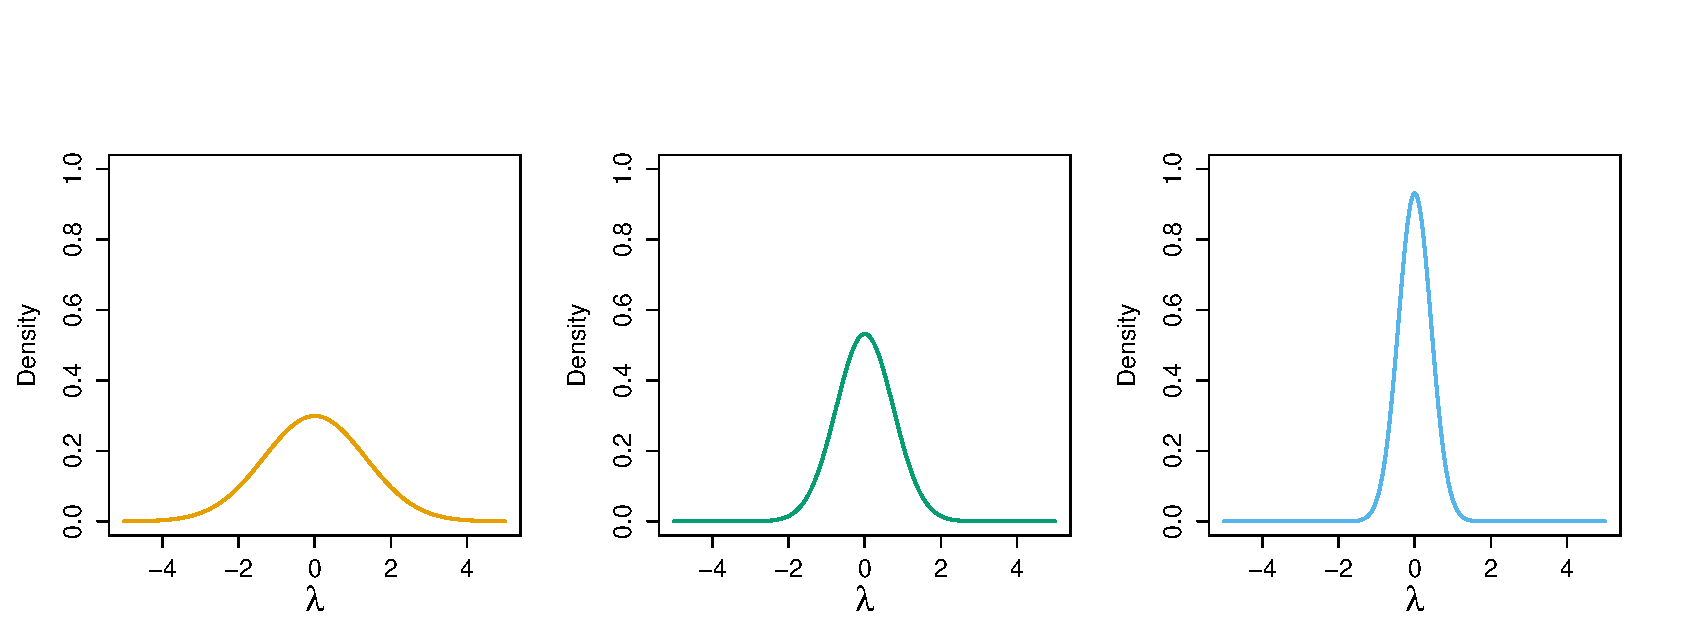
\includegraphics[width=0.6\textwidth, keepaspectratio]{Priors}
	\label{PriorPlot}
\end{figure}

\subsection[Defining new MGP Full Conditionals]{Defining new MGP Full Conditionals}
We propose a Gibbs sampler for posterior computation, much like the one above, and an adaptive strategy for inference on the truncation level $q^\star$ is described in Section \ref{Adapt_Section}. For now, let's focus on the new full conditionals for the loadings matrix, global shrinkages, and local shrinkages which need to be derived in order to implement this. Other full conditionals are exactly as before, with just a small adjustment to the factor scores to allow for the truncation to $q^\star$ columns, i.e. $\mathrm{P}\left(\underline{\eta}_i \given \mbox{---}\right) \sim  \textrm{MVN}_{q^\star}\left(\left[\mathcal{I}_{q^\star} + \Lambda^T_{q^\star}\Psi^{-1}\Lambda_{q^\star}\right]^{-1}\Lambda^T\Psi^{-1}\underline{x}_i - \underline{\mu},\left[\mathcal{I}_{q^\star} + \Lambda^T_{q^\star}\Psi^{-1}\Lambda_{q^\star}\right]^{-1}\right)$

\subsubsection[Loadings Matrix]{Loadings Matrix - $\Lambda$}
Incorporating the new prior \eqref{eq:21}, and following the same steps as Section \ref{Loadings_Section} above, it's trivial to show that the $\Lambda_j$s now have independent conditionally conjugate posteriors given by$\colon$
\begin{equation}
\mathrm{P}\left(\Lambda_j\given \mbox{---}\right) \sim \textrm{MVN}_{q^\star}\left(\left[\mathrm{D}_j^{-1} + \psi_j^{-1}\eta^T\eta\right]^{-1}\eta^T\psi_j^{-1}\underline{x}^{j^\star},\left[\mathrm{D}_j^{-1} + \psi_j^{-1}\eta^T\eta\right]^{-1}\right)\label{eq:24}\end{equation}
\noindent However, we can reintroduce $\underline{\mu}$ and save on computational time, as before, if we follow the routine given in \eqref{eq:16}, with $\Omega_{\lambda_j} = \mathrm{D}_j^{-1} + \psi_j^{-1}\eta^T\eta$.


\subsubsection[Local Shrinkage]{Local Shrinkage -- $\phi_{jk}$}
Using the conditional prior in \eqref{eq:21} and the reparameterised version of \eqref{eq:22}, the prior for $\phi_{jk}$, we can derive the full conditional for the local shrinkage parameter as follows$\colon$
\begin{flalign}
\mathrm{P}\left(\phi_{jk} \given \mbox{---}\right) \propto \mathrm{P}\left(\lambda_{jk} \given \phi_{jk},\tau_k\right)\mathrm{P}\left(\phi_{jk}\right)&\propto \frac{\phi_{jk}^{\nicefrac{1}{2}}\tau_k^{\nicefrac{1}{2}}}{\sqrt{2\pi}}\exp\left\{-\frac{1}{2}\lambda_{jk}^2\phi_{jk}\tau_k\right\}\phi_{jk}^{\nu}\exp\left\{-\nu\phi_{jk}\right\}\nonumber\\
&\propto \phi_{jk}^{\nicefrac{1}{2}}\phi_{jk}^{\nu}\exp\left\{\left(-\frac{1}{2}\lambda_{jk}^2\tau_k - \nu\right)\phi_{jk}\right\}\nonumber\\
&\propto \phi_{jk}^{\nu + \nicefrac{1}{2}}\exp\left\{-\frac{1}{2}\left(2\nu + \lambda_{jk}^2\tau_k\right)\phi_{jk}\right\}\nonumber
\shortintertext{Thus the full conditional for each $\phi_{jk}$ is given by$\colon$}
\mathrm{P}\left(\phi_{jk}\given \mbox{---}\right) &\sim \textrm{Ga}\left(\nu + \frac{3}{2},\nu + \frac{\tau_k\lambda_{jk}^2}{2}\right)\label{eq:26}
\end{flalign}

\subsubsection[Global Shrinkage]{Global Shrinkage -- $\tau_k$}
Using the conditional prior in \eqref{eq:21} and the prior for $\tau_k$ in \eqref{eq:23} we can derive the full conditional for the global shrinkage parameter, in three stages -- first by deriving and sampling from $\mathrm{P}\left(\delta_1\given\mbox{---}\right)~\&~\mathrm{P}\left(\delta_k\given\mbox{---}\right)$ for $k\geq 2$, as follows below --- and then obtaining the product $\tau_k = \prod_{h=1}^k \delta_h$ thereafter$\colon$
\begin{flalign}
\mathrm{P}\left(\delta_1 \given \mbox{---}\right) & \propto \prod_{j=1}^{p}\prod_{k=1}^{q^\star}\textrm{N}\left(\lambda_{jk}\given 0, \phi_{jk}^{-1}\tau_k^{-1}\right) \times \textrm{Ga}\left(\delta_1 \given \alpha_1, \beta_1\right)\nonumber\\
&\propto \prod_{j=1}^p \textrm{N}\left(\lambda_{j1}\given 0, \phi_{j1}^{-1}\tau_1^{-1}\right)\times\ldots\times\prod_{j=1}^p\textrm{N}\left(\lambda_{jq^\star}\given 0, \phi_{jq^\star}^{-1}\tau_{q^\star}^{-1}\right)\times \textrm{Ga}\left(\delta_1\given\alpha_1, \beta_1\right)\nonumber\\
&\propto \left(\phi_{j1}\tau_1\right)^{\nicefrac{p}{2}}\exp\left(-\frac{1}{2}\sum_{j=1}^p\lambda_{j1}^2\phi_{j1}\tau_1\right)\times\ldots\times\left(\phi_{jq^\star}\tau_{q^\star}\right)^{\nicefrac{p}{2}}\exp\left(-\frac{1}{2}\sum_{j=1}^p\lambda_{jq^\star}^2\phi_{jq^\star}\tau_{q^\star}\right)\nonumber\\&\hspace{108mm}\times \delta_1^{\alpha_1-1}\exp\left(-\beta_1\delta_1\right)\nonumber\\
&\propto \left(\phi_{j1}\delta_1\right)^{\nicefrac{p}{2}}\exp\left(-\frac{1}{2}\sum_{j=1}^p\lambda_{j1}^2\phi_{j1}\delta_1\right)\times\ldots\times\left(\phi_{jq^\star}\delta_1\delta_2\ldots\delta_{q^\star}\right)^{\nicefrac{p}{2}}\exp\left(-\frac{1}{2}\sum_{j=1}^p\lambda_{jq^\star}^2\phi_{jq^\star}\delta_1\delta_2\ldots\delta_{q^\star}\right)\nonumber\\&\hspace{135mm}\times \delta_1^{\alpha_1-1}\exp\left(-\beta_1\delta_1\right)\nonumber\\
&\propto\delta_1^{\nicefrac{pq^\star}{2}+\alpha_1-1}\exp\left(-\frac{\delta_1}{2}\left(\sum_{j=1}^p\lambda_{j1}^2\phi_{j1}+\ldots+\lambda_{jq^\star}^2\phi_{jq^\star}\delta_2\ldots\delta_{q^\star} +2\beta_1\right)\right)\nonumber\\
&\propto\delta_1^{\nicefrac{pq^\star}{2}+\alpha_1-1}\exp\left(-\frac{\delta_1}{2}\left(\sum_{h=1}^{q^\star}\tau_h^{\left(1\right)}\sum_{j=1}^p\lambda_{jh}^2\phi_{jh}+2\beta_1\right)\right)\nonumber\\
\mbox{where}~\tau_h^{\left(k\right)} &= \prod_{t=1}^h \frac{\delta_t}{\delta_k}~\mbox{for}~k=1,\ldots,q^\star\label{eq:27}\\
\therefore \mathrm{P}\left(\delta_1\given\mbox{---}\right)& \sim \textrm{Ga}\left(\alpha_1 + \frac{pq^\star}{2}, \beta_1 + \frac{1}{2}\sum_{h=1}^{q^\star}\tau_h^{\left(1\right)}\sum_{j=1}^p\lambda_{jh}^2\phi_{jh}\right)\label{eq:28}
\end{flalign}
\begin{flalign}
\mathrm{P}\left(\delta_k \given \mbox{---}\right) & \propto \prod_{j=1}^{p}\prod_{k=1}^{q^\star}\textrm{N}\left(\lambda_{jk}\given 0, \phi_{jk}^{-1}\tau_k^{-1}\right) \times \textrm{Ga}\left(\delta_k \given \alpha_2, \beta_2\right)\nonumber\\
&\propto \left(\phi_{j1}\delta_1\right)^{\nicefrac{p}{2}}\exp\left(-\frac{1}{2}\sum_{j=1}^p\lambda_{j1}^2\phi_{j1}\delta_1\right)\times\ldots\times\left(\phi_{jq^\star}\delta_1\delta_2\ldots\delta_{q^\star}\right)^{\nicefrac{p}{2}}\exp\left(-\frac{1}{2}\sum_{j=1}^p\lambda_{jq^\star}^2\phi_{jq^\star}\delta_1\delta_2\ldots\delta_{q^\star}\right)\nonumber\\&\hspace{134mm}\times \delta_k^{\alpha_2-1}\exp\left(-\beta_2\delta_k\right)\nonumber\\
&\propto \delta_k^{\nicefrac{p}{2}\left(q^\star - k + 1\right) + \alpha_2 - 1}\exp\left(-\frac{\delta_k}{2}\left(\sum_{h=k}^{q^\star}\tau_h^{\left(k\right)}\sum_{j=1}^p\lambda_{jh}^2\phi_{jh} + 2\beta_2\right)\right)\nonumber\\
\therefore \mathrm{P}\left(\delta_k\given \mbox{---}\right) &\sim \textrm{Ga}\left(\alpha_2 + \frac{p}{2}\left(q^\star - k + 1\right),\beta_2 +\frac{1}{2}\sum_{h=k}^{q^\star}\tau_h^{\left(k\right)}\sum_{j=1}^p\lambda_{jh}^2\phi_{jh}\right)\label{eq:29}
\end{flalign}
\subsection[Adaptive Step]{Adaptive Step}
\label{Adapt_Section}
In practical situations, relatively few important factors are expected compared to the dimension $p$ of the data. The most common approach for selecting the number of factors relies on fitting the finite factor model for different choices of $q^\star$, and then using the BIC, BIC-MCMC, or other model selection criteria. This approach can be difficult to implement for $N \ll p$ problems, and the BIC itself isn't well justified for factor models even for small to moderate $p$. Furthermore, the question of which criterion to use as a basis for model choice is often itself a fraught choice. 

However, the infinite factor model obviates the need for pre-specifying $q^\star$, while the sparsity favouring prior on the loadings ensures that the effective number of factors is small when the truth is sparse. However, we need a computational strategy for choosing an appropriate truncation level that strikes a balance between missing important factors by choosing $q^\star$ too small and wasting computational effort on an overly high truncation level. One can think of $q^\star$ as the effective number of factors, so that the contribution from adding additional factors is negligible. 

Starting with a very conservative guess $\tilde{q}$ as an upper bound for $q^\star$, posterior samples of $\Lambda_{\tilde{q}}$ from the Gibbs sampler contain information about $q^\star$. At the $t$-th iteration, let $m^{\left(t\right)}$ denote the number of columns in $\Lambda_{\tilde{q}}$ having all elements in a pre-specified small neighbourhood of zero. Intuitively, $m^{\left(t\right)}$ of the factors have a negligible contribution at the $t$-th iteration. We then define $q^{\star\left(t\right)} = \tilde{q} - m^{\left(t\right)}$ to be the effective number of factors at iteration $t$. Ideally, we would like to discard redundant factors and continue sampling with fewer loadings columns, to reduce wasted computational effort by discarding unimportant factors. Hence, the algorithm described in Section \ref{Gibbs1} above is modified to an adaptive Gibbs sampler, which tunes the number of factors as it progresses. 

We begin with a default $\tilde{q}$ value of $\min\left(\left\lfloor 3\ln(p)\right\rfloor, p, N-1\right)$. We adapt only after the burn-in period, in order to ensure we're sampling from the true posterior distribution before truncating the loadings matrix. We adapt with probability $\mathrm{p}\left(t\right) = \exp\left(b_0 + b_1t\right)$ at the $t$-th iteration, with $b_0$, $b_1$ chosen so that adaptation occurs often at the beginning of the chain but decreases in frequency exponentially fast after burn-in. We fixed $b_0$ and $b_1$ at $-0.1$ and $-5 \times 10^{-5}$ respectively. We generate a sequence $u_t$ of uniform random numbers between $0$ and $1$. If $u_t \leq \mathrm{p}\left(t\right)$, we monitor the columns in the loadings matrix having $75\%$ of elements less than $10^{-1}$ in magnitude. If the number of such columns drops to zero, an additional loadings column is added by simulating from the prior distribution. Otherwise redundant columns are discarded and parameters corresponding to non-redundant columns are retained. Other parameters are also modified accordingly.

Unlike the PGMM family of models and \citet{Bhattacharya2011}, we allow $q^{\star}$ to shrink all the way to 0, thereby allowing a diagonal covariance structure. Letting $\tilde{q}^{\left(t\right)}$ denote the truncation level at iteration $t$ and $q^{\star\left(t\right)} = \tilde{q}^{\left(t\right)} - m^{\left(t\right)}$ denote the effective number of factors, we use the posterior mode or median of $q^{\star\left(t\right)}$ after burn-in and thinning as an estimate of $q^\star$ with credible intervals quantifying uncertainty. Thus a histogram approximation to the posterior distribution of $q^\star$ is introduced and may be used to address the question about the effective number of latent factors.

\section[Extension to Mixture Modelling]{Extension to Mixture Modelling}
\subsection[Introducing Mixture Models]{Introducing Mixture Models}
Marginally, \eqref{eq:5} provides a parsimonious covariance matrix, i.e.~$\underline{x}_i\given \theta \sim  \textrm{MVN}_p\left(\underline{\mu},\Lambda\Lambda^T + \Psi\right)$.
This allows us to exploit model-based clustering capabilities in high dimensional data settings. We can employ a(n)~(in)finite mixture of factor analyis models whereby each of the $G$ clusters is modelled using a cluster specific latent Gaussian model with covariance specified according to the form above. Let's now introduce some basic notation at this stage: 
\begin{flalign}
N &=\sum_{g=1}^{G}n_g~\quad\hspace{18mm}~\mbox{where $n_g$ is the size of the $g$-th group.}\nonumber\\
\mathrm{P}\left(X\given\gamma\right) &= \sum_{g=1}^{G}\pi_g\mathrm{P}_g\left(X\given\theta_g\right)~\quad\mbox{where}~\gamma = \left(\theta_1,\ldots,\theta_G,\pi_1,\ldots,\pi_G\right),\\
&\hspace{41mm}\mbox{and the p.d.f $\mathrm{P}_g$ is parametrized by $\theta_g$.}\nonumber
\intertext{The \textit{cluster mixing proportions} - $\pi_1,\ldots,\pi_G$ - have the following properties}
\pi_g &\geq~0~\quad\forall~g = 1,\ldots,G\nonumber\\
\sum_{g=1}^{G}\pi_g &= 1\nonumber
\intertext{Introduce an additional latent indicator $G$-vector of \textit{cluster labels} -- $\underline{z}_i$ -- s.t.}
z_{ig} & =
\begin{cases} 1~\mbox{if}~i \in g\\
0~\mbox{otherwise}\end{cases}\nonumber\\
\intertext{Therefore, if $G=3$, for instance, and observation $i$ belongs to cluster 2, $\underline{z}_i =\left(0,1,0\right)$. Hence,} \underline{x}_i\given z_{ig} = 1 &\sim\textrm{MVN}_p\left(\underline{\mu}_g,\Lambda_g\Lambda_g^T + \Psi_g\right)\nonumber\\
\therefore \mathrm{P}\left(\underline{x}_i\right) &= \sum_{g=1}^{G}\pi_g\textrm{MVN}_p\left(\underline{\mu}_g,\Lambda_g\Lambda_g^T + \Psi_g\right)\label{eq:30}
\end{flalign}
\subsubsection[Decomposable Prior for $\gamma$]{Decomposable Prior for $\gamma$}
\begin{flalign}
\shortintertext{The posterior distribution of $\gamma$ is}
\mathrm{P}\left(\gamma\given X\right) & \propto \mathrm{P}\left(\gamma\right)\prod_{i=1}^{N}\mathrm{P}\left(\underline{x}_i\given\gamma\right)\nonumber\\
&\propto \mathrm{P}\left(\gamma\right)\prod_{i=1}^{N}\left(\sum_{g=1}^{G}\pi_g\mathrm{P}_g\left(\underline{x}_i\given\theta_g\right)\right)\nonumber\\
\therefore \mathrm{P}\left(\gamma\given X,Z\right) & \propto \mathrm{P}\left(\gamma\right)\prod_{g=1}^{G}\prod_{i\colon z_{ig} = 1}\mathrm{P}_g\left(\underline{x}_i\given\theta_g\right)\nonumber
\shortintertext{If $\mathrm{P}\left(\gamma\right)$ can be decomposed into}
\mathrm{P}\left(\gamma\right) &= \mathrm{P}\left(\pi\right)\prod_{g=1}^{G}\mathrm{P}\left(\theta_g\right)\mbox{, then}\nonumber\\
\mathrm{P}\left(\gamma\given X,Z\right) & \propto \mathrm{P}\left(\pi\right)\prod_{g=1}^{G}\prod_{i\colon z_{ig}=1}\mathrm{P}\left(\theta_g\right)\mathrm{P}_g\left(\underline{x}_i\given \theta_g\right) \label{eq:31}
\end{flalign}
\subsection[Deriving Posterior Distributions]{Deriving Posterior Distributions}
Attention now turns towards deriving full conditional distributions for the new parameter $\underline{\pi}$, as well as the latent variables $Z$, so that we can sample them for clustering purposes, by incorporating them into the Adaptive Gibbs Sampler framework described variously above.

\begin{itemize}
	\item Component Parameters -- $\theta_g\colon$	\vspace{2mm}\\
	$\mathrm{P}\left(\theta_g\given\theta_{-g},X,Z\right) \equiv \mathrm{P}\left(\theta_g\given X,Z\right) \propto \prod_{i\colon z_{ig} = 1}\mathrm{P}\left(\theta_g\right)\mathrm{P}_g\left(\underline{x}_i\given\theta_g\right)$\vspace{2mm}\\
	where $\theta_{-g} = \left(\theta_1,\ldots,\theta_{g-1},\theta_{g+1},\ldots,\theta_G\right)$\\
	\item Cluster Mixing Proportions -- $\underline{\pi}\colon$\vspace{2mm}\\
	$\mathrm{P}\left(\underline{\pi}\given X, Z\right) \equiv \mathrm{P}\left(\underline{\pi}\given Z\right) \propto \mathrm{P}\left(\underline{\pi}\right)\prod_{g=1}^{G}\pi_g^{n_g}$\vspace{2mm}\\
	where $n_g$ is the number of observations in group $g$,\vspace{2mm}\\
	since $\mathrm{P}\left(\underline{z}_i\given\underline{\pi}\right) \sim \textrm{Mult}\left(1, \underline{\pi}\right)$\\
	\item Latent Variables -- $\underline{z}_i\colon$\vspace{2mm}\\
	$\mathrm{P}\left(\underline{z}_i\given\underline{x}_i,\gamma\right) \propto \mathrm{P}\left(\underline{z}_i\right)\mathrm{P}\left(\underline{x}_i\given\theta_{i\colon z_{ig}=1},\underline{z}_i\right)$
\end{itemize}
\subsubsection[Cluster Mixing Proportions]{Cluster Mixing Proportions -- $\underline{\pi}$}
\label{pi_prior}
Let the prior distribution of $\underline{\pi}$ be Dirichlet with parameter $\underline{\alpha}$ -- a multivariate generalisation of the Beta distribution. Typically an exchangeable symmetric uniform prior is chosen, whereby $\alpha_g = 1~\forall~g=1,\ldots,G$.
\begin{flalign}
\mathrm{P}\left(\underline{\pi}\right) &\propto \prod_{g=1}^{G}\pi_g^{\alpha_g-1}\nonumber\\
\therefore \mathrm{P}\left(\underline{\pi}\given Z, X\right) & \propto \prod_{g=1}^{G}\pi_g^{\alpha_g-1}\prod_{g=1}^{G}\pi_g^{n_g}\nonumber\\
&\propto \prod_{g=1}^{G}\pi_g^{\alpha_g + n_g - 1}\nonumber\\
\mbox{i.e.}~\mathrm{P}\left(\underline{\pi}\given Z, X\right) &\sim \textrm{Dir}\left(\underline{\alpha}+\underline{n}\right)\label{eq:32}\\
\mbox{where}~\underline{n} &= \left(n_1,\ldots,n_G\right)\nonumber
\end{flalign}
\subsubsection[Latent Variables]{Latent Variables -- $\underline{z}_i$}
\begin{flalign}
\underline{z}_i \given \underline{x}_i,\gamma &\sim \textrm{Mult}\left(1,\underline{p}\right),~\mbox{where}\nonumber\\
\underline{p} &= \left(p_1,\ldots,p_G\right),~\mbox{and}\nonumber\\
p_g &=~\mathrm{P}\left(z_{ig}=1\given\underline{x}_i,\gamma\right) = \frac{\pi_g\mathrm{P}\left(\underline{x}_i\given\theta_g\right)}{\sum_{g=1}^{G}\pi_g\mathrm{P}\left(\underline{x}_i \given\theta_g\right)} = \frac{\pi_g f\left(\underline{x}_i \given \underline{\mu}_g,\Lambda_g\Lambda_g^T+\Psi_g\right)}{\sum_{g=1}^G\pi_g f\left(\underline{x}_i \given \underline{\mu}_g,\Lambda_g\Lambda_g^T+\Psi_g\right)}\label{eq:33}&\\
&=\exp\Big[\log\left(\pi_g\right) + \log\Big(f\big(\underline{x}_i \given \underline{\mu}_g,\Lambda_g\Lambda_g^T+\Psi_g\big)\Big) - \sum_{g=1}^{G}\left(\log\left(\pi_g\right) + \log\Big(f\big(\underline{x}_i \given \underline{\mu}_g,\Lambda_g\Lambda_g^T+\Psi_g\big)\right)\Big]\nonumber
\end{flalign}
\newpage
\subsubsection[Mixtures of Infinite Factor Analyzers Pseudo-Code]{Mixtures of Infinite Factor Analyzers Pseudo-Code}

MIFA has the dual advantages of allowing different clusters to be modelled by different numbers of latent factors, and significantly reducing the model search to one for $G$ only, as $q_g$ is estimated during model fitting.
\begin{enumerate}[label*=\arabic*.]
	\item Choose hyperparameters as before and initialise cluster labels $Z^{\left(0\right)}\colon$~by simulation from the $\textrm{Mult}\left(1, \underline{\pi}\right)$ prior, or employ other clustering algorithms, such as K-Means or Mclust. Compute $\underline{n}$, and $\underline{\tilde{\mu}}_g$ for each group.
	\item Initialise, $\forall~g=1,\ldots,G\colon$
		\begin{flalign}
	\underline{\mu}_g^{\left(0\right)} &\sim \textrm{MVN}_p\left(\underline{\tilde{\mu}}_g, \Sigma_{\mu}\right) &\nonumber\\
	\underline{\eta}_{i}^{\left(0\right)} &\sim\textrm{MVN}_{q_g^\star}\left(\underline{0},\mathcal{I}_{q_g^\star}\right)~\quad\forall~i = 1,\ldots,N&\nonumber\\
	\underline{\Lambda}_{jg}^{\left(0\right)} &\sim\textrm{MVN}_{q_g^\star}\left(\underline{0},\Sigma_{\lambda}\right)~\quad\hspace{1.5mm}\forall~j = 1,\ldots,p&\nonumber\\
	\psi_{jg}^{-1^{\left(0\right)}} &\sim \textrm{Ga}\left(\alpha,\beta_j\right)~\quad\quad\hspace{5mm}\forall~j = 1,\ldots,p&\nonumber\\
	\phi_{jkg}^{\left(0\right)} &\sim \textrm{Ga}\left(\nu + 1,\nu\right)~\qquad\forall~j = 1,\ldots,p\quad\mbox{and}\quad k=1,\ldots,q_g^\star\nonumber\\
	\delta_{1g}^{\left(0\right)} &\sim \textrm{Ga}\left(\alpha_1,\beta_1\right),\hspace{3mm}\delta_{hg}^{\left(0\right)} \sim \textrm{Ga}\left(\alpha_2,\beta_2\right),\quad h\geq 2\nonumber\\
	\tau_{kg}^{\left(0\right)} &= \prod_{h=1}^{k}\delta_{hg}^{\left(0\right)}\quad\hspace{17mm}\forall~k=1,\ldots,q_g^\star\nonumber
		\end{flalign}
	\item For $g = 1,\ldots,G$, sample other parameters as before, but this time from their \textit{group specific} full conditionals$\colon$
	\begin{alignat*}{4}
		\alphloop&\Omega_{\mu_g}^{\left(t\right)} &=&~\Sigma_{\mu}^{-1} + n_g\Psi_g^{-1^{\left(t-1\right)}}\\
		&\underline{\mu}_g^{\left(t\right)} &\sim&~\textrm{MVN}_p\left(\Omega_{\mu_g}^{-1^{\left(t\right)}}\Big(\Psi_g^{-1^{\left(t-1\right)}}\big(\sum_{i\colon z_{ig} = 1}\underline{x}_i - \sum_{i\colon z_{ig} = 1}\Lambda_g^{\left(t-1\right)}\underline{\eta}_i^{\left(t-1\right)}\big) + \Sigma_{\mu}^{-1}\underline{\tilde{\mu}}_g\Big),\Omega_{\mu_g}^{-1^{\left(t\right)}}\right)\\
		\alphloop&\Omega_{\eta_g}^{\left(t\right)} &=&~\mathcal{I}_{q_g^\star} + \Lambda_g^{T^{\left(t-1\right)}}\Psi_g^{-1^{\left(t-1\right)}}\Lambda_g^{\left(t-1\right)}\\
		&\underline{\eta}_{i\colon z_{ig} = 1}^{\left(t\right)}~&\sim&~\textrm{MVN}_q\left(\Omega_{\eta_g}^{-1^{\left(t\right)}}\Lambda_g^{T^{\left(t-1\right)}}\Psi_g^{-1^{\left(t-1\right)}}\left(\underline{x}_{i\colon z_{ig} = 1} -\underline{\mu}_g^{\left(t\right)}\right),\Omega_{\eta_g}^{-1^{\left(t\right)}}\right)\\
		\alphloop &\mbox{For}~j &=& 1, \ldots, p\\
		\bullet~&\Omega_{\lambda_{jg}}^{\left(t\right)} &=& \mathrm{D}_j^{-1} + \psi_{jg}^{-1^{\left(t-1\right)}}\eta_{i\colon z_{ig} = 1}^{T^{\left(t\right)}}\eta_{i\colon z_{ig} = 1}^{\left(t\right)}\\
		&  \underline{\Lambda}_{jg}^{\left(t\right)} &\sim& \textrm{MVN}_{q_g^\star}\left(\Omega_{\lambda_{jg}}^{-1^{\left(t\right)}}\eta_{i\colon z_{ig} = 1}^{T^{\left(t\right)}}\psi_{jg}^{-1^{\left(t-1\right)}}\left(\underline{x}_{i\colon z_{ig} = 1}^j -\underline{1}\mu_{jg}^{\left(t\right)}\right),\Omega_{\lambda_{jg}}^{-1^{\left(t\right)}}\right)\\
		\bullet~&  \psi_{jg}^{-1^{\left(t\right)}} &\sim& \textrm{Ga}\left(\alpha + \frac{n_g}{2},\beta_j + \frac{S_{jg}^{\left(t\right)}}{2}\right)\\
		\bullet~& \phi_{jkg}^{\left(t\right)} &\sim& \textrm{Ga}\left(\nu + \frac{3}{2},\nu+\frac{\tau_{kg}^{\left(t-1\right)}\lambda_{jkg}^{2^{\left(t\right)}}}{2}\right)\quad\forall~k=1,\ldots,q_g^\star\\
		\alphloop&\delta_{1g}^{\left(t\right)} &\sim& \textrm{Ga}\left(\alpha_1 + \frac{pq_g^\star}{2},\beta_1 + \frac{1}{2}\sum_{h=1}^{q_g^\star}\tau_{hg}^{\left(1\right)^{\left(t-1\right)}}\sum_{j=1}^p\lambda_{jhg}^{2^{\left(t\right)}}\phi_{jhg}^{\left(t\right)}\right)\\
		&\delta_{hg}^{\left(t\right)} &\sim& \textrm{Ga}\left(\alpha_2 + \frac{p}{2}\left(q_g^\star-k+1\right), \beta_2 + \frac{1}{2}\sum_{h=k}^{q_g^\star}\tau_{hg}^{\left(k\right)^{\left(t\right)}}\sum_{j=1}^p\lambda_{jhg}^{2^{\left(t-1\right)}}\phi_{jhg}^{\left(t\right)}\right),\quad h\geq 2\\
		&\tau_{kg}^{\left(t\right)} &=& \prod_{h=1}^{k}\delta_{hg}^{\left(t\right)}\quad\hspace{38mm}\forall~k=1,\ldots,q_g^\star\nonumber
		\end{alignat*}
	\item Re-compute $\underline{n}$, sample $\underline{\pi}$ from $\textrm{Dir}\left(\underline{\alpha} + \underline{n}\right)$ and sample $\underline{z}_i$ as outlined in \eqref{eq:33}.
	\item Follow the adaptation procedure outlined in Section \ref{Adapt_Section}.
	\item Repeat steps 4--7 for $t=2,\ldots,T$ using the current value for $q_g^\star$.
	\item Disregard the first $\textrm{B}$ burn-in iterations and thin every $\textrm{K}$-th iteration \footnote{With MFA, one chooses between competing models according to the pair of G and q values which optimise any of the model selection criteria outlined in Section \ref{Gibbs1}. With MIFA, one chooses G using BICM or AICM only.}.
\end{enumerate}
\subsection[Label Switching]{Label Switching}
It's easy to see that $\mathrm{P}\left(X\given\gamma\right) = \mathrm{P}\left(X\given\tilde\gamma\right)$ where $\tilde\gamma = \left(\theta_{j_1},\ldots,\theta_{j_G},\pi_{j_1},\ldots,\pi_{j_G}\right)$ and $j_1,\ldots,j_G$ is any permutation of $1,\ldots,G$. This type of finite mixture distribution nonidentifiability is caused by the invariance of mixture distributions to component relabelling: by interchanging the order of components, the distributions induced by $\gamma$ and $\tilde{\gamma}$ are the same, although evidently the two parameters are distinct. For finite mixture distribution as defined above with $G$ components, there exist $G!$ equivalent ways of arranging them. Generally as the Markov chain progresses, we will observe switches between these equivalent modes. When the main goal is identifying/interpreting mixture components \&/or clustering, this \textit{label switching} phenomenon needs to be addressed. The approach we adopt to do so is applied post-hoc, after the chain has finished running, and has the advantage of not involving loss functions based on sampled model parameters. We only require samples of $Z$, which are matched to a template vector of cluster labels at burnin using the cost-minimizing permutation suggested by the square assignment algorithm \citep{CarpToth1980}. This same permutation is applied to all other parameters which vary by group, namely the means, loadings, uniquenesses, and mixing proportions, prior to computing their posterior mean estimates.

\subsection[Overfitted Mixtures]{Overfitted Mixtures}
The need to choose the optimal number of latent factors in a mixture of factor analysers has been obviated using MIFA, but the issue of model choice is still not entirely resolved. Overfitted mixtures, along with Dirichlet processes (Section \ref{Dirichlet}) and transdimensional MCMC, are a means of extending the MIFA method in order to estimate $G$ in a similarly choice-free manner. The prior in Section \ref{pi_prior}  plays an important role. Mixture model estimation is approached by initially overfitting the number of clusters expected to be present, and specified conditions on the Dirichlet hyperparameter vector $\underline{\alpha}$ for the  mixing proportions encourage the emptying out of excess components in the posterior distribution. 

To initialise the method, a conservatively high number of groups $G^\star = \max\left(\left\lfloor 3\ln(N)\right\rfloor, 25, N-1\right)$ is chosen, and fixed for the entire length of the MCMC chain. It's assumed that $G^\star > G$. Each $\alpha_g = 0.5/G^\star$ is set small enough to favour empty groups a priori \citep{Ishwaran2001}. The symmetric uniform prior $\textrm{Dir}\left(1,\ldots,1\right)$ used previously is rather indifferent in this respect. The number of non-empty groups at each iteration $G_0$ is recorded thusly:
\begin{equation}
	G_0 = G^{\star} - \sum_{g=1}^{G} \mathbbm{1}\big(\sum\limits_{i} z_{ig}=0\big)\label{eq:34}
\end{equation}
\label{overfitted}
The true $G$ is estimated by the $G_0$ value visited most often by the sampler. Component specific inference is conducted only on the $M_0$ samples corresponding to those visits. However, this method is not ideal in the sense that there is a conflict of opinion on `how small' $\alpha$ needs to be: too large and no/few clusters will be emptied, too large and the estimate will shrink close to the true $G$, but mixing proportions will become so small that new clusters will rarely be formed. Furthermore, the sampler needs to carry round and simulate empty groups from priors, with the adaptation scheme modified to exclude empty groups about which we have no information.

\section[Dirichlet Process Mixture Models]{Dirichlet Process Mixture Models}
\label{Dirichlet}

Traditional mixtures of factor analyzers using a fixed and finite number of components and factors can suffer from over and under-fitting, where there is a misfit between the complexity of the model and the amount of data available. Model selection is a difficult issue and it involves the double and interdependent choice of number of factors and number of mixture components. The proposed MIFA model represents an alternative to parametric modeling by allowing theoretically infinitely many factors. IMIFA is a similarly Bayesian nonparametric extension to MIFA designed to address the issue of determining the number of clusters, $G$, by allowing infinitely many of them through a Dirichlet process prior, thereby yielding a `choice-free' approach which obviates the need for model selection criteria. In so doing, it represents also a way to sidestep the fraught task of determining the number of model parameters, bringing significant flexibility. It must be noted that, even if theoretically the number of mixture components is infinite under a Dirichlet process prior, practically they are at most equal to the sample size $N$, if we ignore empty components, and the growth rate of $\mathbb{E}\left(G\right)$ is known to be logarthmic in $N$. In the same way the infinite factor model detailed above can retain a number of effective factors at most equal to the number of variables $P$ in practice, by ignoring redundant factors.

\subsection[Dirichlet Processes]{Dirichlet Processes}
Dirichlet processes are stochastic processes whose draws are random probability measures. A probability distribution $H$ is a Dirichlet process with parameters $H_0$, the \textit{base distribution}, and $\alpha$, the \textit{concentration parameter}, denoted $H \sim \textrm{DP}\left(\alpha, H_0\right)$, if every marginal of $H$ on finite partitions of the domain $\Omega$ are Dirichlet distributed, as per the following definition due to \citet{Ferguson1973}:
\begin{flalign}
	\left(H\left(A_1\right),\ldots,H\left(A_r\right)\right) &\sim \textrm{Dir}\left(\alpha H_0\left(A_1\right),\ldots,\alpha H_0\left(A_r\right)\right)\label{eq:35}\\
	A_1\cup\ldots\cup A_r &= \Omega\nonumber\intertext{The base distribution $H_0$ can be interpreted as the prior guess for the parameters of the model or the mean of the DP:}
	\mathbb{E}\left[H(A)\right] &= H_0(A)\label{eq:36}\intertext{The concentration parameter $\alpha$ expresses the strength of belief in $H_0$:}
	\mathbb{V}\left[H(A)\right] &= \dfrac{H_0(A)(1-H_0(A))}{\alpha+1}\label{eq:37}
\end{flalign}

The choice of the base distribution for the model parameters is important for the model performance. In our implementation, the base distribution comes from the factor analytic structure given variously above. This allows us define the general model $f\left(\underline{x}_i\right)=  \sum_{g=1}^{\infty}\pi_g\textrm{MVN}_p\left(\underline{\mu}_g, \Lambda_g\Lambda_g^\top + \Psi_g\right)$. We consider conjugate prior distributions for the model parameters, with additional layers for the hyperparameters, as specified above. 

There exist several equivalent metaphors which motivate methods of yielding samples from a DP without representing the infinite dimensional variable $G$ explicitly, which make its key properties more clear, e.g. Chinese Restaurant Process, P\'olya-Urn Scheme, and Stick-Breaking Representation. We focus on the latter. Furthermore, MCMC sampling strategies can be divided into two families; marginal methods, which integrate out the infinite dimensional probability measure $H$ and directly represent the partition structure of the data e.g. \citep{Escobar1994, EscWest1995, Neal2000}, as well as conditional methods, which sample a sufficient but finite number of groups at each iteration, e.g. truncation \citep{Ishwaran2001}, retrospective sampling \citep{Papaspiliopoulos2008}, and slice sampling \citep{Walker2007, Kalli2011}. We adopt the latter approach.

\subsection[Stick-Breaking Construction]{Stick-Breaking Construction}
The stick-breaking construction of \citet{Sethuraman1994} metaphorically views the mixing proportions $\left\{\pi_1,\pi_2, \ldots\right\}$ as pieces of a unit-length stick that is sequentially broken in an infinite process, with stick-breaking proportions $\left\{V_1, V_2, \ldots\right\}$ according to realisations of a Beta distribution, and can be summarised as follows:
\begin{flalign}
V_g  &\sim \textrm{Beta}(1,\alpha) &\theta_g &\sim H_0\nonumber&\\
\pi_g    &=V_g \prod_{l=1}^{g-1}(1-V_l) &H &=\sum_{g=1}^\infty \pi_g \delta_{\theta_g} \sim \textrm{DP}\left(\alpha, H_0\right)\label{eq:38}
\end{flalign}
where
$\delta_\theta$ is the Dirac delta centered at $\theta$ and $\theta=\left\{\underline{\mu},\Lambda,\Psi\right\}$ denotes the whole set of parameters of the cluster-specific \textrm{FA} models, s.t. draws are composed of a sum of infinitely many point masses. We use this as a prior process for generating the weights of the infinite mixture distribution.

\subsection[Slice Sampling]{Slice Sampling}
The slice sampler of \citet{Walker2007} introduces an auxiliary variable $u > 0$ which preserves the marginal distribution of the data $x$ and facilitates writing the conditional density of $x \given u$ as a finite mixture, by letting $\underline{\xi}=\left\{\xi_1, \xi_2, \ldots\right\}$ be a decreasing sequence of infinite quantities which sum to $1$, s.t. the joint distribution of $\left(x,u\right)$ is 

\begin{flalign} 
f(x,u\given\theta, \underline{\xi})&=\sum_{g=1}^\infty \pi_g\textrm{Unif}(u; 0, \xi_g) f(x;\theta_g)\label{eq:39}\shortintertext{with}
f(x;\theta)&=\int f(x,u) du\hspace{3mm}=\sum_{g=1}^\infty \pi_g f(x;\theta_g) \int \textrm{Unif}(u; 0, \xi_g) du=\sum_{g=1}^\infty \pi_g f(x;\theta_g)\label{eq:40}\shortintertext{and}
f(u;\underline{\xi})&= \int f(x,u;\theta,\underline{\xi})=\sum_{g=1}^\infty \pi_g \textrm{Unif}(u; 0, \xi_g) \int f(x;\theta_g) dx=\sum_{g=1}^\infty \pi_g \textrm{Unif}(u; 0, \xi_g) = \sum_{g=1}^\infty \dfrac{\pi_g}{\xi_g} \indicator{u<\xi_g}\label{eq:41}\shortintertext{Since only a finite number of $\xi_g$ are greater than $u$, by denoting $\mathcal{A}_\xi\left(u\right)=\{g: u < \xi_g\}$, the conditional density of $x \given u$ can be written as a \textit{finite} mixture model:}
f\left(x \given u;\theta\right)&= \frac{f\left(x,u;\theta,\underline{\xi}\right)}{f\left(u;\underline{\xi}\right)}\hspace{2.5mm}=\sum_{g \in \mathcal{A}_\xi\left(u\right)}\frac{\pi_g}{\xi_g f\left(u;\underline{\xi}\right)} f\left(x;\theta_g\right)\label{eq:42}\shortintertext{because}
\textrm{Unif}\left(u; 0, \xi_g\right) &= \frac{1}{\xi_g}\indicator{u <\xi_g}\nonumber \\
\mbox{Now}~f\left(\underline{x}_i\right)&=  \sum_{g=1}^{\infty}\pi_g\textrm{MVN}_p\left(\underline{\mu}_g, \Lambda_g\Lambda_g^\top + \Psi_g\right)~\mbox{can be sampled from}.\nonumber
\end{flalign}
Typically $\xi_g = \pi_g$, but `independent' slice-efficient sampling \citep{Kalli2011} allows for a deterministic decreasing sequence, e.g. geometric decay $\xi_g=\left(1-\rho\right)\rho^{g-1}$,where $\rho$ is a fixed value $\boldsymbol\in \left(0, 1\right)$. The $\rho$ parameter must be chosen delicately; higher values will lead to better mixing, but longer running times, since the size of the set $\mathcal{A}_\xi\left(u\right)$ increases. We find $\rho=0.75$ strikes an appropriate balance. For slice sampling, components and corresponding parameters are reordered at each iteration such that the mixing proportions form a decreasing sequence.

\subsection[Infinite Mixtures of Infinite Factor Analysers]{Infinite Mixtures of Infinite Factor Analysers}
We impose a hierarchical structure on the latent variables and parameters which utilizes the auxiliary variable of the independent slice efficient sampler, with geometric
decay values. The joint
distribution of the factor-analytic mixture-model with infinite components is proportional to:
\begin{eqnarray}
	f\left(x,\eta,z,\underline{u},\underline{V},\theta\right)&\propto& f\left(x \given \eta,z,\underline{u},\underline{V},\theta\right)f\left(\eta \given \underline{u}\right)f\left(z,\underline{u} \given \underline{V},\underline{\pi}\right)f\left(\underline{V} \given \alpha\right)f\left(\theta\right) \nonumber\\
	&\propto & \left\{\prod_{i=1}^N \prod_{g \in \mathcal{A}_\xi\left(u_i\right)} \textrm{MVN}_p\left(x_i; \underline{\mu}_g + \Lambda_g\underline{\eta}_{i}, \Psi_g\right)^{z_{ig}}\right\} \nonumber\\
	&&\left\{\prod_{i=1}^N \prod_{g \in \mathcal{A}_\xi\left(u_i\right)} \textrm{MVN}_q\left(\underline{\eta}_{i};0,\mathcal{I}_q\right)\right\} \nonumber\\
	&& \left\{ \prod_{i=1}^N \prod_{g=1}^\infty \left(\dfrac{\pi_g}{\xi_g} \indicator{u_i<\xi_g}\right)^{z_{ig}}\right\} \left\{ \prod_{g=1}^\infty \dfrac{(1-V_g)^{\alpha-1}}{\textrm{Beta}\left(1,	\alpha\right)}\right \}f(\theta)\label{eq:43}
\end{eqnarray}

\noindent where $f(\theta)$ is the full collection of conjugate priors defined previously, under the trick that only the `active components' such that $g \in  \mathcal{A}_\xi\left(u_i\right)$ have to be estimated. Thus the number of active components which have to be estimated at each iteration is given by $G=\max_{1 \leq i \leq N} \vert\mathcal{A}_\xi\left(u_i\right)\vert$, where $\vert\mathcal{A}_\xi\left(u_i\right)\vert$ is the cardinality of $\mathcal{A}_\xi\left(u_i\right)$. This discrete number varies but is fixed at each iteration, even if theoretically infinite. However, it's the non-empty subset rather than active clusters that are of interest. As with the OMIFA model in Section \ref{overfitted}, the algorithm is initialised with a conservatively high starting value for the number of groups, above the truth in the spirit of \citet{Hastie2014}, and the true G is estimated by the number of non-empty clusters visited most often, with cluster-specific inference is
conducted only on samples corresponding to those visits. All conditional posteriors have standard form and the IMIFA algorithm can proceed via efficient Gibbs updates. 

\subsection[IMIFA Full Conditionals]{IMIFA Full Conditionals}
\begin{flalign}
\intertext{From \eqref{eq:43}}
\underline{V} \given \mbox{---}    &\propto  \prod_{g=1}^\infty \pi_g^{n_g}  (1-V_g)^{\alpha-1}=\prod_{g=1}^\infty V_g^{n_g} \left(\prod_{l<g}(1-V_l) \right)^{n_g}  (1-V_g)^{\alpha-1}\nonumber\intertext{The previous expression can be expanded as:}
\underline{V} \given \mbox{---}   &\propto V_1^{n_1} (1-V_1)^{\alpha-1} V_2^{n_2} (1-V_1)^{n_2} (1-V_2)^{\alpha-1} V_3^{n_3} (1-V_1)^{n_3} (1-V_2)^{n_2} (1-V_3)^{\alpha-1}\nonumber\\
&\phantom{=~}V_4^{n_4} (1-V_1)^{n_4} (1-V_2)^{n_4} (1-V_3)^{n_4} (1-V_4)^{\alpha-1} \ldots \nonumber\\ 
& = V_1^{n_1} (1-V_1)^{\alpha -1} (1-V_1)^{N-n_1}  V_2^{n_2} (1-V_2)^{\alpha -1} (1-V_2)^{N-n_1-n_2} \ldots\nonumber\intertext{from which for $V_g$}
V_g \given \mbox{---}  &\sim \textrm{Beta}\left(1+n_g,\alpha+N-\sum_{l=1}^g n_l \right)\label{eq:44}
\end{flalign}

\noindent To derive a full conditional for the auxiliary variable $u_i$, observe that $f\left(z, \underline{u}\given \underline{V}, \underline{\pi}\right)$ in \eqref{eq:43} can be rewritten as $f\left(\underline{z}_i, u_i \given \underline{V}, \underline{\pi}\right) = f\left(\underline{z}_i, u_i\given \underline{\pi}\right) = \prod_{g=1}^{\infty}\left(\pi_g\textrm{Unif}\left(u;0,\xi_g\right)\right)^{z_{ig}}$ because the weights $\underline{\pi}$ are deterministic functions of $\underline{V}$. We thus derive the full conditional for $u_i$ as:
\begin{equation}
u_i\given z_{ig}=1 \sim \textrm{Unif}\left(0, \xi_g\right)\label{eq:45}
\end{equation}

\newpage\noindent From \eqref{eq:33} and \eqref{eq:43}, it is straightforward to show that 
\begin{equation}
	z_{ig}=1\given \mbox{---} \propto \pi_g\mathrm{P}\left(\underline{x}_i\given\theta_g\right)\frac{\pi_g}{\xi_g}\indicator{u_i < \xi_g}= \pi_g f\left(\underline{x}_i \given \underline{\mu}_g,\Lambda_g\Lambda_g^T+\Psi_g\right)\frac{\pi_g}{\xi_g}\indicator{u_i < \xi_g}\label{eq:46}
\end{equation}
Though it remains fixed in many applications, we also add a $\textrm{Ga}\left(a, b\right)$ prior for the concentration parameter $\alpha$, according to the auxiliary variable routine of \citet{West1992} reproduced below, so that it can be learned from the data.
\begin{flalign}
	\textrm{P}\left(G\given \alpha, N\right)&\propto \alpha^{G-1}\dfrac{\left(\alpha + N\right)\beta\left(\alpha + 1, N\right)}{\Gamma\left(N\right)}\qquad\qquad\footnotesize{(G=1,\ldots,N)}\nonumber&\\
	\therefore \alpha \given G, \chi &\sim \omega_\chi \textrm{Ga}\left(a + G, b - \log\left(\chi\right)\right) + \left(1 - \omega_\chi\right)\textrm{Ga}\left(a + G - 1, b - \log\left(\chi\right)\right)\label{eq:47}
\end{flalign}
with weights defined by: $\dfrac{\omega_\chi}{1 - \omega_\chi} = \dfrac{\left(a + G - 1\right)}{N\left(b - \log\left(\chi\right)\right)}$, \newline
where $\beta$ is the Beta function
and $\left(\chi \given \alpha, G\right) \sim \textrm{Beta}\left(\alpha + 1, N\right)$.\newline

Finally, as state spaces for real data IMIFA applications can be highly multimodal, with well separated regions of high posterior probability coexisting, corresponding to clusterings of different sizes, we incorporate the label switching moves suggested by \citet{Papaspiliopoulos2008}. These are complimentary moves which are effective at swapping similar and unequal clusters, respectively. Parameters are reordered accordingly after each accepted move.

\begin{itemize}
	\item Change labels of two randomly chosen non-empty clusters $g$ and $h$ with probability:\\ \quad $\min \left\{1, \left(\nicefrac{\pi_h}{\pi_g}\right)^{n_g - n_h}\right\}$
	\item Change labels of neighbouring non-empty clusters $g$ and $g+1$ with probability:\\ \quad$\min\left\{1, \nicefrac{\left(1-V_{g}\right)^{n_g}}{\left(1-V_{g+1}\right)^{n_{g+1}}}\right\}$
\end{itemize}

\section[Results]{Results}
\subsection[Simulation Study]{Simulation Study}
A simulation study with the following design was conducted in order to assess IMIFA's performance: data with $G=3$ groups and $p=50$ variables was simulated according to the factor analytic structure, with $q_g=4$ latent factors in each group. To evaluate performance in different dimensionality scenarios, this was done with $N=25, 50~\mbox{and}~300$. Groups are roughly balanced and also quite close, in terms of the small difference in their location parameters. Sensitivity to the concentration parameter $\alpha$ is examined by running the model at various fixed values, and by allowing $\alpha$ to be learned according to \eqref{eq:46}. In order to reduce error due to simulation, results are based on repeating the study over ten replicate datasets meeting the same criteria. With 12,500 iterations, with the first 2,500 discarded due to burn-in and every 2\textsuperscript{nd} sample thinned, this gives 50,000 samples contributing to each row of the aggregated table below. The quantities in brackets are 95\% credible intervals.\newline

\footnotesize
\centering
\begin{tabular}[pos=center]{I c | c I c | c | c | c I c | c I}
	\specialrule{.1em}{.01em}{.01em}
	\centering
	\textbf{Dimension} & $\boldsymbol{\alpha}$ & \textbf{G} & $\mathbf{q_1}$ & $\mathbf{q_2}$ & $\mathbf{q_3}$ & 	{\centering\textbf{Time (s)}} & {\centering\textbf{Error (\%)}}\\
	\specialrule{.1em}{.01em}{.01em}
	\multirow{4}{0.1\linewidth}{\centering N = 25\quad(N~$\ll$~p)} & 0.5 & 3 [3,3] & 4 [2,8] & 4 [2,8] & 4 [2,8] & 327.03 & 0\\
	& 1 & 3 [3,3] & 4 [2,8] & 4 [2,8] & 4 [2,8] & 328.11 & 0\\
	& 5 & 3 [3,4] & 4 [2,8] & 4 [2,8] & 4 [2,8] & 330.50 & 0\\
	& Learned & 3 [3,3] & 4 [2,8] & 3 [2,7] & 4 [2,8] & 327.56 & 0\\
	\hline
	\label{SimulationStudy}
	\multirow{4}{0.1\linewidth}{\centering N = 50\quad(N~$=$~p)} & 0.5 & 3 [3,3] & 5 [3,6] & 5 [3,6] & 5 [3,7] & 361.66 & 0\\
	& 1 & 3 [3,3] & 5 [3,7] & 5 [3,7] & 5 [3,7] & 363.06 & 0\\
	& 5 & 3 [3,3] & 5 [3,6] & 5 [3,6] & 4 [3,7] & 367.44 & 0\\
	& Learned & 3 [3,3] & 5 [3,6] & 5 [3,6] & 5 [3,7] & 366.57 & 0\\
	\hline
	\multirow{4}{0.1\linewidth}{\centering N = 300\qquad(N $\gg$ p)} & 0.5 & 3 [3,3] & 5 [4,6] & 5 [4,6] & 5 [4,6] & 555.82 & 0\\
	& 1 & 3 [3,3] & 5 [4,6] & 5 [4,6] & 5 [4,6] & 558.52 & 0\\
	& 5 & 3 [3,3] & 5 [4,6] & 5 [4,6] & 5 [4,6] & 560.75 & 0\\
	& Learned & 3 [3,3] & 5 [4,6] & 5 [4,6] & 5 [4,6] & 560.46 & 0\\
	\specialrule{.1em}{.01em}{.01em}
\end{tabular}

\justifying
\normalsize
This demonstrates good performance in the sense that the modal estimate of $G$ uncovered the truth in all cases, with only the scenario with $N \ll P$ and $\alpha$ fixed too large showing some deviation in the $95\%$ credible interval. Furthermore, estimates of $q_g$ are within the limits of the credible intervals in every case also. Lastly, clustering performance is perfect. Overall, the IMIFA model demonstrates excellent ability to uncover the truth of simulated data.

\subsection[Olive Oil Benchmark]{Olive Oil Benchmark}
Further assessment of IMIFA's clustering performance was conducted using data from \citet{Forina1983} on the percentage composition of 8 fatty acids found by lipid fraction of 572 Italian olive oils, from three areas: Southern Italy, Sardinia, and Northern Italy. Within each area there are a number of different regions. Southern Italy comprises North Apulia, Calabria, South Apulia, and Sicily. Sardinia is divided into Inland Sardinia and Coastal Sardinia. Northern Italy comprises Umbria, East Liguria, and West Liguria. As such the true number of groups is hypothesised to correspond to either 3 \textit{areas} or 9 \textit{regions}. The full suite of models, from (Infinite) Factor Analysis through Mixtures of (Infinite) Factor Analysers, to (Overfitted/Infinite) Mixtures of (Infinite) Factor Analysers, were run on the data for 50,000 iterations, with the first 10,000 discarded and every 2\textsuperscript{nd} sample thereafter thinned. Results for methods that rely on ranges of $G$ and/or $q$ values being supplied are based on $G=1,\ldots,9$, and $q=0,\ldots,6$, respectively, with the optimal model chosen by BICM where necessary. The results are summarised in the table below, with clusterings evaluated using the Adjusted Rand Index, and the percentage error rate, compared to the known \textit{area} labels. Though the $\alpha$ parameter plays different roles in each of these models, it is given as its fixed value or posterior mean, as appropriate. The IMIFA algorithm was used as the baseline for the relative time.\newline 

\centering
\footnotesize
\begin{tabular}[pos=center]{I c | c | c | c | c | c | c | c | c I}
	\specialrule{.1em}{.01em}{.01em} 
	\centering
	\label{Olive_Results}
	\textbf{Method} & \textbf{\# Models} & \textbf{Time (s)} & \textbf{Rel. Time} & $\boldsymbol{\alpha}$ & $\mathbf{G}$ & $\mathbf{q}$ & \textbf{Adj. Rand} & \textbf{Error (\%)}\\
	\specialrule{.1em}{.01em}{.01em}
	IMIFA & 1 & 1814.59 & 1.000 & 4.54 & 4 & 6, 2, 3, 2 & 0.9345 & 8.57\\
	IMFA & 7 & 13152.41 & 7.248 & 4.79 & 6 & 5, 5, 5, 5, 5, 5 & 0.5164 & 37.24\\
	OMIFA & 1 & 1860.42 & 1.025 & 0.025 & 5 & 6, 2, 2, 2, 2 & 0.9037 & 15.91\\
	OMFA & 7 & 9547.15 & 5.261 & 0.025 & 6 & 5, 5, 5, 5, 5, 5 & 0.5153 & 37.41\\
	MIFA & 9 & 6848.13 & 3.774 & 1 & 1 & 6 & 0 & 43.53\\
	MFA & 63 & 33636.22 & 18.537 & 1 & 2 & 5, 5 & 0.8192 & 17.13\\
	IFA & 1 & 240.82 & 0.133 & -- &  1 & 6 & -- & --\\
	FA & 7 & 1092.95 & 0.602 & -- &  1 & 6 & -- & --\\
	\specialrule{.1em}{.01em}{.01em} 
\end{tabular}
\justifying
\normalsize
\newline

Of the 572 observations, 323 originate in Southern Italy. This large cluster requires the largest amount of factors. It's clear that the flexibility to model remaining clusters by lower numbers of factors greatly improves clustering performance. Indeed, the best solution is given by IMIFA, which requires only one run and doesn't rely on any model selection criteria. The IMIFA performance compares favourably to the PGMM solution also, which gives a 5 group, 5 factor model (Adj. Rand = 0.5586, Error Rate = 33.56). It's also worth noting that the optimal models chosen by algorithms which do rely on model selection criteria were not all optimal in a clustering sense -- for instance, in this case where the `truth' is known, the candidate MIFA model with $G=4$ yields an Adj. Rand of 0.9304 and an error rate of 10.49\%, despite having a non-optimal BICM. The cross tabulation of the MAP clustering from the IMIFA model against the known area labels suggests the possibility of a fourth group, whereby Umbria is separated from East and West Liguria in the North. This makes sense, geographically. The confusion matrix using this relabelling yields an Adj. Rand of 0.9961 and an error rate of 0.7\%. Indeed, the other methods also perform better with this labelling.
\begin{table}[H]
	\footnotesize
	\caption{IMIFA olive oil confusion matrices}
	\begin{minipage}{.5\linewidth}
		\centering
		\begin{tabular}[pos=left]{c | c | c | c | c}
			& 1 & 2 & 3 & 4 \\
			\specialrule{.1em}{.01em}{.01em} 
			South & 323 & 0 & 0 & 0\\
			Sardinia & 0 & 97 & 1 & 0\\
			North & 0 & 0 & 103 & 48 \\
		\end{tabular}		
	\end{minipage}%
	\begin{minipage}{.5\linewidth}
		\centering
		\begin{tabular}[pos=left]{c | c | c | c | c}
			& 1 & 2 & 3 & 4 \\
			\specialrule{.1em}{.01em}{.01em} 
			South & 323 & 0 & 0 & 0\\
			Sardinia & 0 & 97 & 1 & 0\\
			Liguria & 0 & 0 & 100 & 0\\
			Umbria & 0 & 0 & 3 & 48
		\end{tabular}
	\end{minipage} 
	\label{Olive_Clustering}
\end{table}
\justifying

In order to assess the IMIFA algorithm's robustness, $\mathrm{N}\left(0,1\right)$ noise with no classification information was appended separately to the rows and columns of the Olive data, generating 6 new scenarios with 10, 50 and 100 extra variables, and the same number of extra observations, respectively. Cluster validity is evaluated with respect to the new 4-group relabelling: in the case of extra rows, new observations are labelled as though they belonged to a fifth group. Data were centered and scaled prior to expansion. Runtime is given relative to the IMIFA run on the original data.

\begin{center}
\begin{tabular}[pos=center]{I c | c | c | c | c | c | c I}
	\specialrule{.1em}{.01em}{.01em} 
	\centering
	\label{Olive_Robust}
	\textbf{Scenario} & \textbf{Rel. Time} & $\boldsymbol{\alpha}$ & $\mathbf{G}$ & $\mathbf{q}$ & \textbf{Adj. Rand} & \textbf{Error (\%)}\\
	\specialrule{.1em}{.01em}{.01em}
	N=572, p=18 & 1.364 & 4.55 & 6 & 2, 2, 2, 2, 2, 2 & 0.9366 & 13.64\\
	N=572, p=58 & 3.121 & 4.55 & 5 & 2, 1, 1, 1, 2 & 0.7365 & 14.69\\
	N=572, p=108 & 5.168 & 4.56 & 4 & 1, 1, 1, 1 & 0.7334 & 17.66\\
	\specialrule{.1em}{.01em}{.01em}
	N=582, p=8 & 1.219 & 4.53 & 11 & 4, 2 $\times$ 10 & 0.8582 & 14.6\\
	N=622, p=8 & 1.225 & 4.48 &  9 & 3, 2 $\times$ 8  & 0.5632  & 30.23 \\
	N=672, p=8 & 2.309  & 4.41  & 7  & 2 $\times$ 7  & 0.6232  & 28.12 \\
	\specialrule{.1em}{.01em}{.01em} 
\end{tabular}
\end{center}
\justifying
The group structure can still be uncovered reasonably well as the number of irrelevant variables increases, however there is increasing support for a 1-group, 1-factor model as the signal-to-noise ratio decreases. As such, variable selection, or at least the need to pre-process the data, may still be an issue. As rows of noise are appended, the algorithm generally has no difficulty in assigning these observations to a group of their own, however their presence is leading to overestimation of the total number of groups, yielding a poorer (though still homogeneous) clustering overall.

\subsection[Real Data]{Real Data}
A real application of IMIFA is given on $N \ll p$ metabolomic data consisting of 189 spectral peaks from urine samples of just 18 subjects, half of which have epilepsy and half of which are controls. Data were mean-centered and scaled by the square root of their standard deviation prior to analysis. This `Pareto' scaling is common practice for metabolomic data \citep{vandenBerg2006}.

\begin{figure}[h]
	\centering
	\caption{Spectral metabolomic data}
	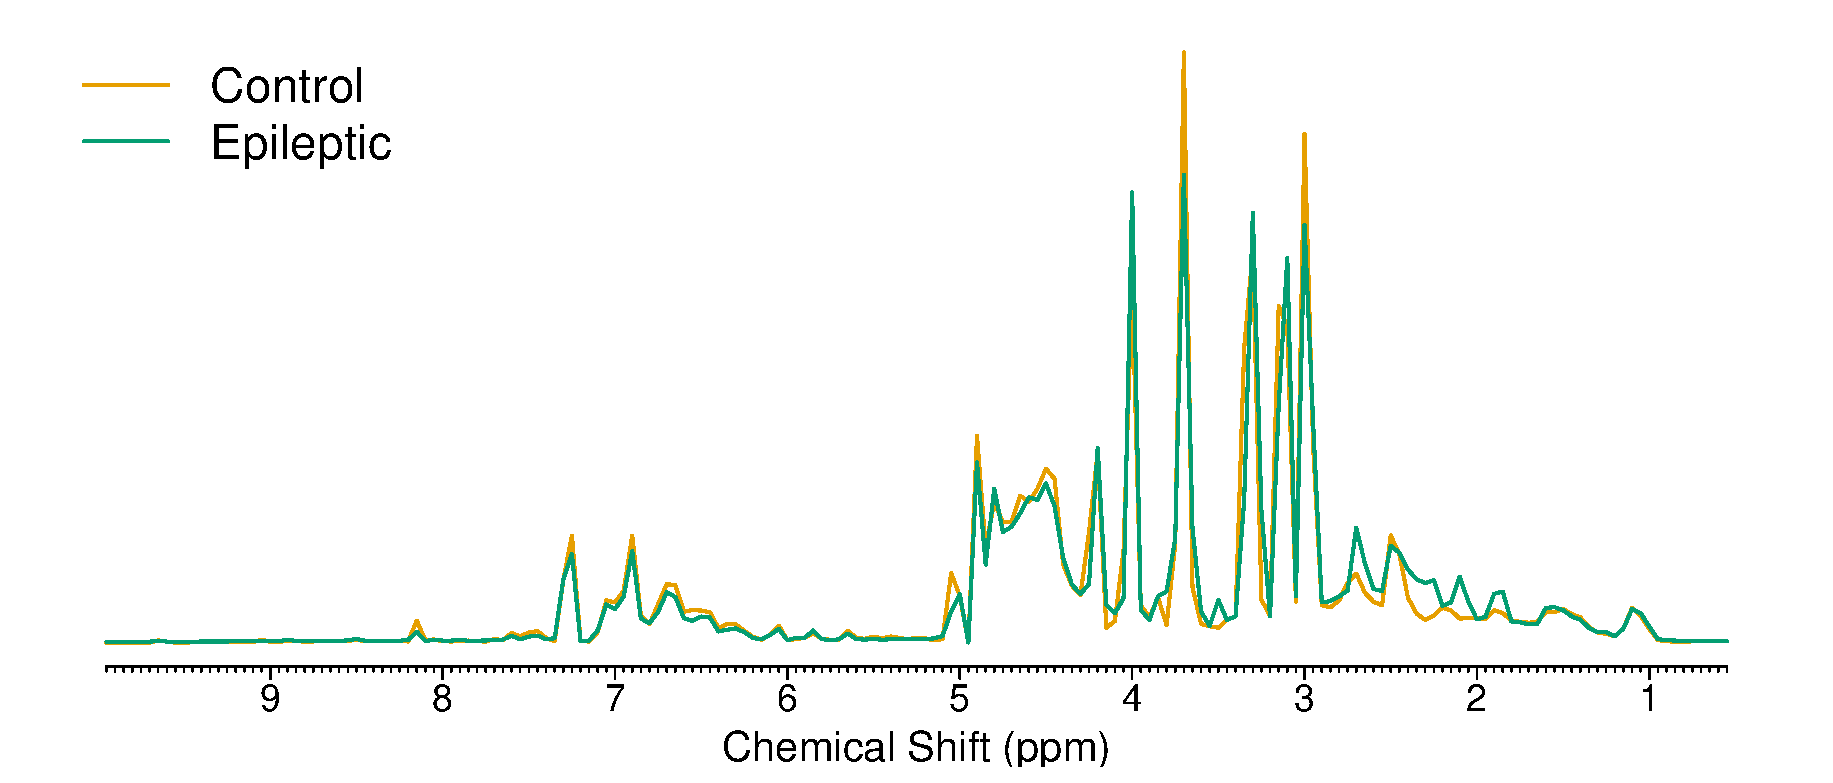
\includegraphics[width=0.7\textwidth, keepaspectratio]{Rat_Data.eps}
	\label{RatData}
\end{figure}

Results are compared against MFA and MIFA runs. To ensure satisfactory convergence, all results are based on 50,000 iterations, with the first 10,000 discarded due to burn-in and every 2\textsuperscript{nd} sample thinned. Cluster labels were initialised using Mclust for all methods \citep{Mclust}. When fitting MFA with $G$ fixed at $2$, over a range of $q$ values from $0,\ldots,10$, BICM suggests $q_g = 3$ for each cluster and 4 observations are misclassified. When fitting MIFA over a range of $G$ values from $1, \ldots, 5$, BICM correctly chooses $2$ as the optimal number of clusters and only one subject is clustered incorrectly. Uncertainty in the number of latent factors for each MIFA cluster is quantified by 95\% credible intervals -- $q_1 \in \left(1,4\right)$ \& $q_2 \in \left(2,5\right)$. It's worth noting the greater complexity in the epileptic cluster. Similarly, heatmaps of each cluster's $p\times q_g$ \textit{posterior mean loadings} matrix, based only on a subset of retained samples with $q_g$ or more factors, after applying Procrustes rotation, demonstrate the sparsity and shrinkage induced by the multiplicative gamma process prior.

\begin{figure}[h]
	\centering
	\begin{subfigure}{0.5\textwidth}
		\centering
		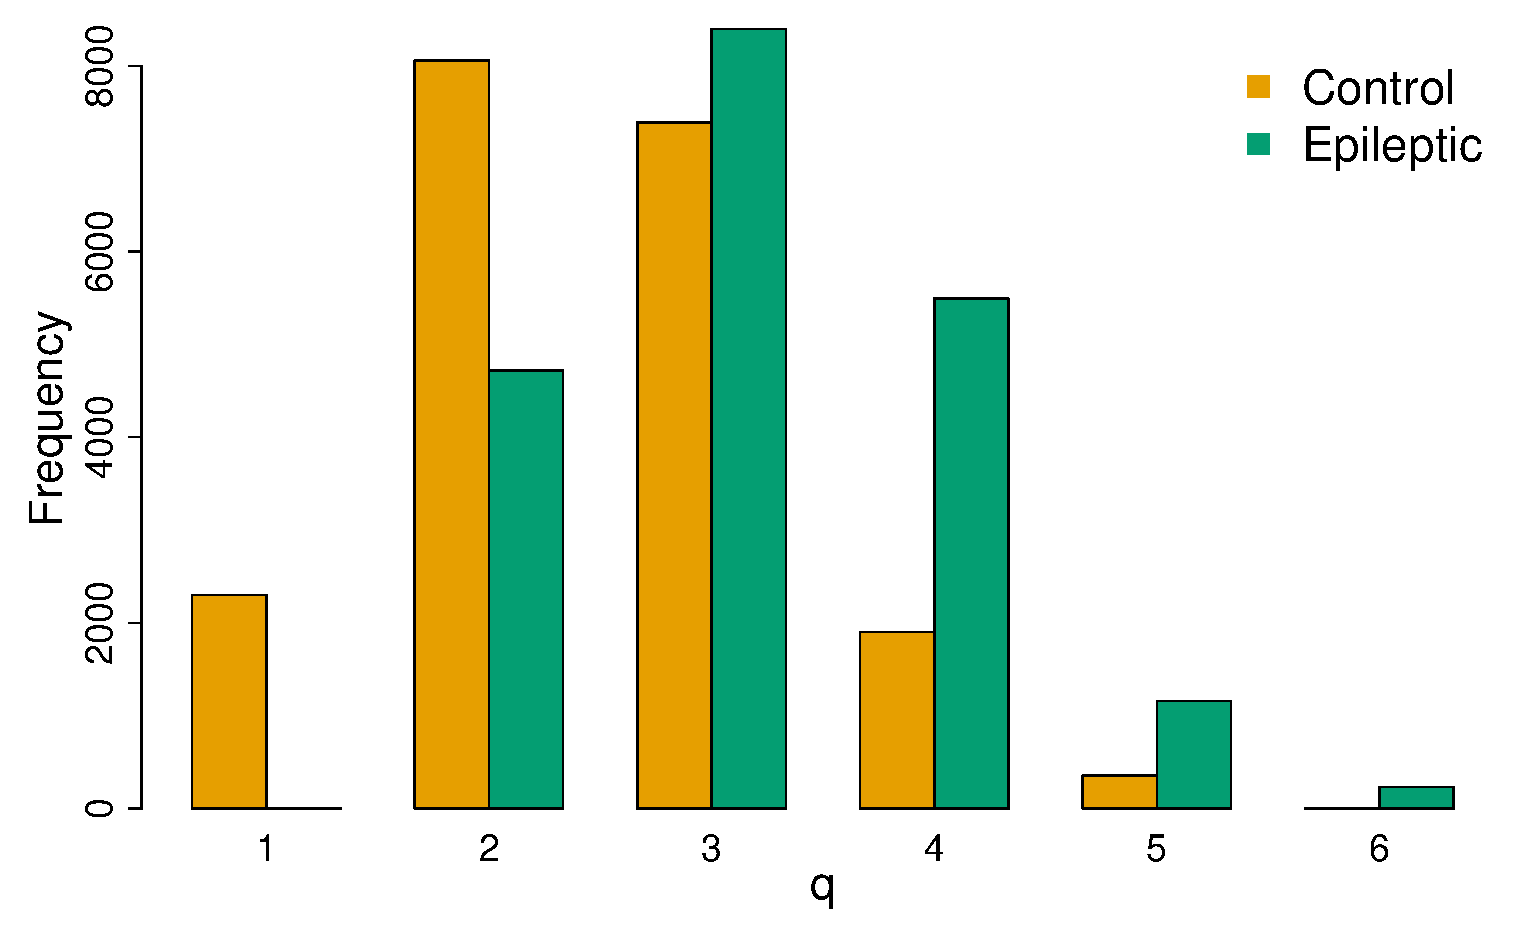
\includegraphics[width=\linewidth, keepaspectratio]{Qdist.eps}
		\caption{Approximation to posterior distribution of $q_g$}
		\label{MIFA_Qdist}
	\end{subfigure}%
	\begin{subfigure}{0.5\textwidth}
		\centering
		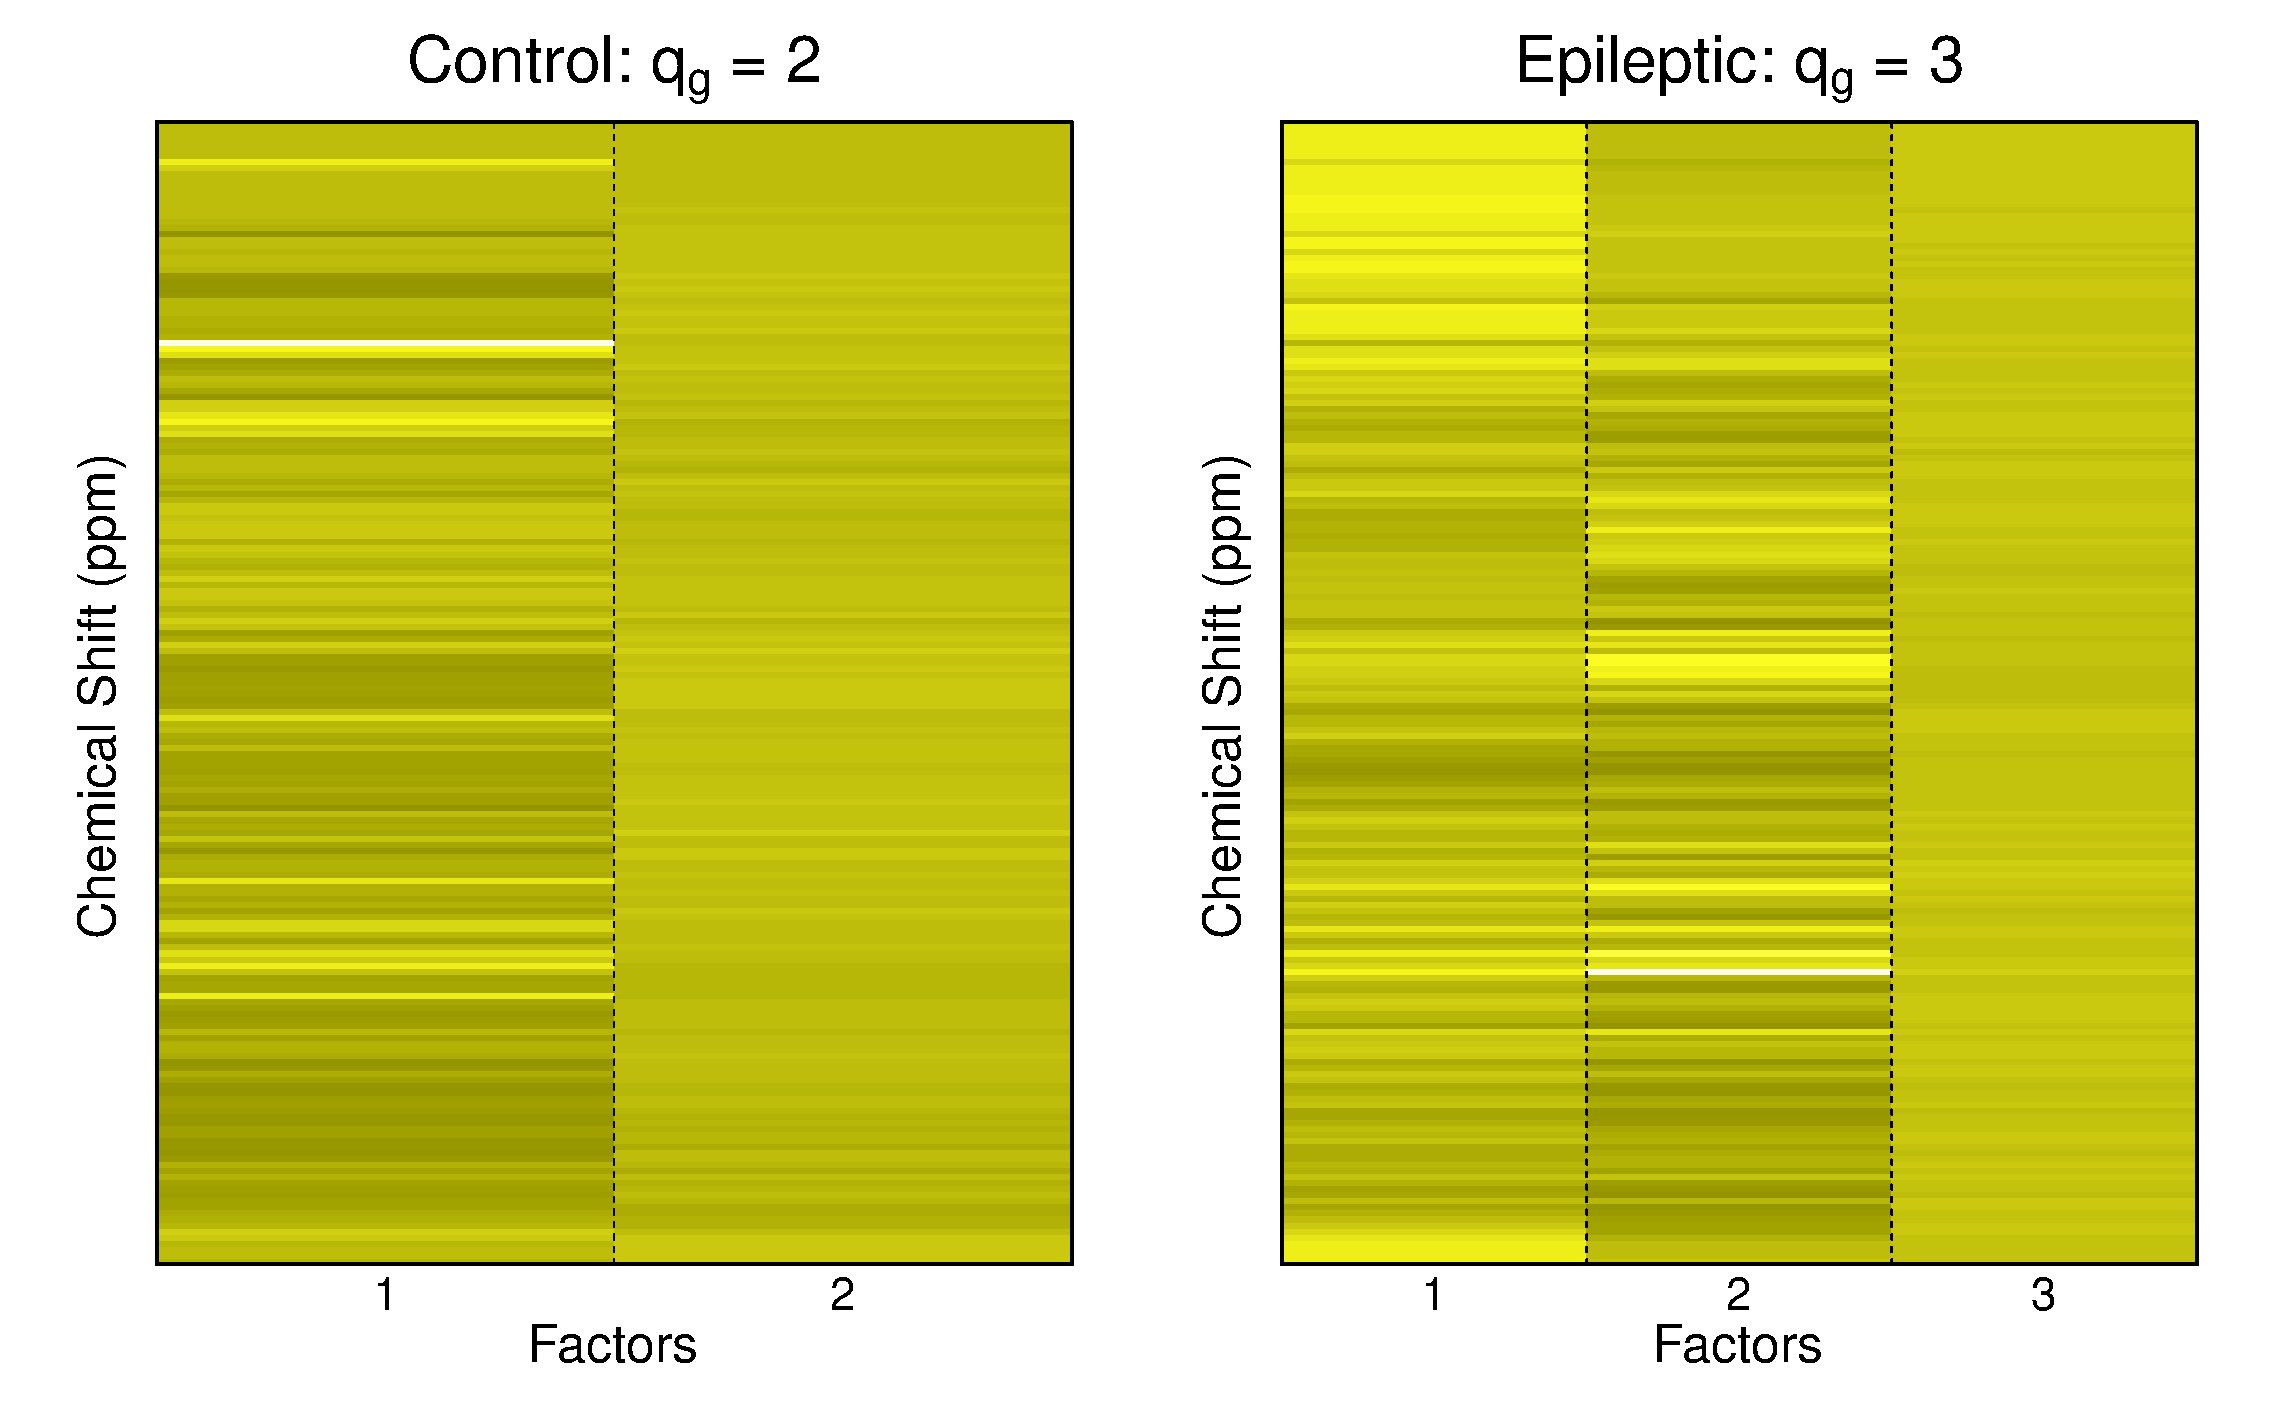
\includegraphics[width=\linewidth, keepaspectratio]{Loadings_Heatmap.eps}
		\caption{Posterion mean loadings matrices heatmaps}
		\label{MIFA_Loadings}
	\end{subfigure}
		\caption{Results on the number of latent factors in two metabolomic MIFA clusters}
		\label{MIFA_UrineResults}
\end{figure}

One run of IMIFA, however, with sufficiently strong shrinkage hyperparameters and $\alpha$ not fixed, is unanimous in visiting a $3$-cluster model in all retained samples, with the modal estimate of $q_g$ in each group being $2$ in each case. The corresponding modal clustering uncovers the cluster structure perfectly, save for the one subject previously misclassified by MIFA now being given its own component. As such, the method may be useful from an outlier detection point of view - indeed, examination of excluded covariates associated with these subjects reveals this epileptic observation to have an abnormally low weight value, quite distinct not only from the other observations in its cluster, but from all observations. Furthermore, perhaps the absence of the outlier in the epileptic cluster accounts for the estimate $q_g$ therein now being $2$, rather than $3$ as it was under MIFA above.

\begin{table}[h]
	\caption{\textbf{IMIFA Metabolomic Clustering}\\ Adj. Rand = 0.8944\\ Error Rate = 5.56\%}
	\centering
	\begin{tabular}[pos=center]{c | c | c | c}
		\centering
		& 1 & 2 & 3 \\
		\specialrule{.1em}{.01em}{.01em} 
		Control & 9 & 0 & 0\\
		Epileptic & 0 & 8 & 1\\
	\end{tabular}
	\label{Urine_Confusion}
\end{table}
\section[Extensions]{Extensions}
The Pitman-Yor process is a popular generalisation of the Dirichlet Process \citep{Perman1992}, and is sometimes referred to as the two-parameter Poisson-Dirichlet process. This prior introduces a discount parameter, $d$, which lies in the interval $\left[0, 1\right)$. In order to satisfy the rules of probability, the $\alpha$ parameter must be strictly greater than $-d$. The PY prior reduces to the Dirichlet process prior when $d=0$. Nonetheless, some important distributional features of the PY process are fundamentally different when this parameter is non-zero. Conveniently, this prior has its own stick-breaking construction, given by
\begin{equation}
V_g \sim \textrm{Beta}\left(1 - d, \alpha + gd\right)\label{eq:48}
\end{equation}
which means this generalisation can be easily incorporated into our Gibbs sampling framework. In particular, non-zero discount has the effect of flattening the Dirichlet process prior and mitigating against its `rich-get-richer' property. The PY prior allows a small number of large groups plus some small groups with the growth rate of $\mathbb{E}\left(G\right)$ now Zipfian rather than logarithmic in $N$. Though the discount parameter remains fixed in our implementation, the gamma prior on $\alpha$ in \eqref{eq:47} is shifted to account for non-zero $d$ values. \newline

\noindent Below are some possible further extensions to this work:
\begin{itemize}
	\item Rewrite code bottlenecks using \pkg{RCPP}.
	\item Investigate block updating the loadings using a matrix normal prior \citep{Viroli2011}. When $q_g$ is fixed, this works, albeit surprisingly slower than current code. It remains to reformulate the MGP prior as a matrix normal. \citet{Bhattacharya2015} could be helpful in this regard.
	\item Implement the third label switching move of \citet{Hastie2014}.
	\item Learn the shrinkage hyperparameters $\alpha_1$ \& $\alpha_2$, which was proposed but not implemented by \citet{Bhattacharya2011}. This requires the introduction of Metropolis-Hastings steps.
	\item \citet{Yu2009} gives a strategy for Collapsed Gibbs Sampling of Dirichlet Process Mixture Models.
	\item The present work could be extended to (semi-)supervised settings where some or all of the data is labelled, in order to use MIFA for (semi-)supervised Model Based Classification.
	\item Covariates could be incorporated in the spirit of Bayesian Factor Regression Models \citep{West2003, Wang2007, Carvalho2008}; for instance, the spectral metabolomic urine data also contains information on weight and urine pH.
	\item The \pkg{IMIFA} package includes functions to assist in soliciting good priors for either Dirichlet or Pitman-Yor processes, by finding the expected number of groups for a given combination of $\alpha$, $N$, and $d$ values, as well as the variance. A third function exists to actually plot the induced distribution on $G$, but at present this is only possible in the case where $d=0$. Extending this function to plot Pitman-Yor priors with non-zero discount requires computation of generalized Stirling numbers of the second kind. Furthermore, $d$ currently remains fixed. Some papers introduce a $\textrm{Beta}\left(1, 1\right)$ prior on it, but strategies for subsequently updating $d\given\mbox{---}$ are unclear, at least in papers I have read to date.
	\item Practically useful extensions to heavier-tailed errors using multivariate $t$ distributions in place of the multivariate normal here are easily encompassed within the simulation based Bayesian analysis we develop and use, as per \citet{Peel2000}. For many applied problems, the tails of the normal distribution are often shorter than required. Also, the estimates of the component means and covariance matrices can be affected by observations that are atypical of the components in the normal mixture model being fitted. The problem of providing protection	against outliers in multivariate data is a very difficult problem and increases with the difficulty of the dimension of the data. With this $t$ mixture model-based approach, the normal distribution for each component in the mixture is embedded in a wider class of elliptically symmetric distributions with an additional parameter called the degrees of freedom $\kappa$. The normal-scale characterisation of the mixture of \textrm{MVt} distributions is given as follows:
	\begin{flalign}
	p_g =~\mathrm{P}\left(z_{ig}=1\given\underline{x}_i,\gamma,\kappa_g\right) &= \frac{\pi_g\mathrm{P}\left(\underline{x}_i\given\theta_g,\kappa_g\right)}{\sum_{g=1}^{G}\pi_g\mathrm{P}\left(\underline{x}_i \given\theta_g,\kappa_g\right)} = \frac{\pi_g f\left(\underline{x}_i \given \underline{\mu}_g,\nicefrac{\left(\Lambda_g\Lambda_g^T+\Psi_g\right)}{U_i}\right)}{\sum_{g=1}^G\pi_g f\left(\underline{x}_i \given \underline{\mu}_g,\nicefrac{\left(\Lambda_g\Lambda_g^T+\Psi_g\right)}{U_i}\right)}\label{eq:49}\shortintertext{where} 
	U_i \given z_{ig} = 1 &\sim \textrm{Ga}\left(\frac{1}{2}\kappa_g,\frac{1}{2}\kappa_g\right)\label{eq:50}
	\end{flalign}
	As $\kappa$ tends to infinity, the $t$ distribution approaches normality, as each $U_i$ will tend to one with probability one. Hence this parameter $\kappa$ may be viewed as a robustness tuning parameter. It can be fixed in advance or it can be inferred from the data for each component.
	\item As results above when appending Gaussian noise to the Olive data show, variable selection, or at least pre-processing of the data, may be still be required.
\end{itemize}
{\small
	\bibliography{Notes_bibtex}}
\end{document}